\documentclass[twocolumn,linenumbers]{aastex631}
\usepackage{rotating}

\renewcommand\labelitemi{{\boldmath$\cdot$}}
\newcommand\tstrut{\rule{0pt}{5.5ex}}
\newcommand\tstrutsmall{\rule{0pt}{5.5ex}}
\newcommand\bstrut{\rule[-6.0ex]{0pt}{0pt}}
\newcommand\bstrutsmall{\rule[-2.5ex]{0pt}{0pt}}
\newcommand{\msun}{$M_{\odot}$}
\newcommand{\logg}{$\log{g}$}
\newcommand{\teff}{${T}_{\mathrm{eff}}$}

\shorttitle{WD+MS Ages}
\shortauthors{Heintz et al.}

\graphicspath{{./}}
\begin{document}

\title{}

\correspondingauthor{Tyler M. Heintz}
\email{tmheintz@bu.edu}

\author[0000-0003-3868-1123]{Tyler M. Heintz}
\affiliation{Department of Astronomy \& Institute for Astrophyiscal Research, Boston University, 725 Commonwealth Ave, Boston, MA, 02215, USA}

\author[0000-0001-5941-2286]{J. J. Hermes}
\affiliation{Department of Astronomy \& Institute for Astrophyiscal Research, Boston University, 725 Commonwealth Ave, Boston, MA, 02215, USA}

\author[0000-0002-4284-8638]{Jennifer L. van Saders}
\affiliation{Institute for Astronomy, University of Hawai’i, 2680 Woodlawn Drive, Honolulu, HI 96822, USA}


\begin{abstract}

\end{abstract}
\keywords{white dwarfs, binary stars, ages, spectroscopy}

\section{Introduction}\label{sec:chap4_intro}
Stellar age is a notoriously difficult parameter to measure but is vital to many areas of astrophysical research. There have been numerous studies over the years developing and improving indirect methods of measuring a star's age (see review by \citealt{2010ARA&A..48..581S}). In parallel with efforts to improve stellar age measurements, many studies using the best available ages have investigated their implications on stellar and galactic evolution. 

It has long been hypothesized and observed that stellar age shows a correlation with metallicity, known as the age-metallicity relation \citep[AMR, ][]{1974A&A....32..321M, 1993A&A...275..101E}. As early generations of stars enrich the galactic medium, more metal-rich stars are able to form. Thus, newly formed stars are expected to have higher metallicities on average. The observed correlation between age and metallicity is often weak and has been debated through the years, with high-metallicity globular clusters posing a challenge \citep[e.g. NGC 6791, ][]{2015ApJ...799..202B} as well as recent comprehensive work showing a relatively flat relation \citep{2014A&A...565A..89B, 2021MNRAS.501.4917W}. Stellar age is found to more strongly correlate with specific elements such as lithium, beryllium, and even uranium \citep[e.g.,][]{2023ApJ...948..122S}, allowing for strong constraints on age to be achieved through these abundances.

It has also been shown that older populations of stars show a larger dispersion in velocity \citep[e.g.,][]{1974A&A....32..321M}. Stars in the galaxy experience interactions with the galactic potential, which effectively heats the population over time, giving rise to an increased velocity dispersion as a function of age. There have been many attempts over the years to constrain the age-velocity dispersion relation \citep[e.g.,][]{2009A&A...501..941H}, including work using white dwarfs \citep{2019ApJ...886..100C} but recent work using white dwarf main-sequence binaries shows a general lack of correlation between age and velocity dispersion \citep{2022A&A...658A..22R}.

White dwarf stars are promising candidates for determining stellar age. Due to their relatively simple cooling and evolution, precise and accurate age determinations are possible. They have been used as chronometers for decades, including being used to age the Galactic disk \citep{1987ApJ...315L..77W} and halo \citep{2019MNRAS.482..965K} and wide binary companions \citep{2019ApJ...870....9F, 2020ApJ...891..171Z}.

With the advent of the Gaia mission \citep{2016A&A...595A...1G,2018A&A...616A...1G,2021A&A...649A...1G}, the number of known white dwarfs has increased substantially \citep{2021MNRAS.508.3877G}, including white dwarfs in wide binary systems \citep{2018MNRAS.480.4884E, Tian, 2021MNRAS.506.2269E}. This provides unprecedented opportunity to test white dwarf ages and utilize them to determine ages of their companions. Recent work has used these wide binaries to constrain the initial-final mass relation \citep{2015ApJ...815...63A, 2024MNRAS.527.9061H} as well as reveal interesting physics at the fully convective boundary of M dwarfs \citep{2024arXiv240312129C}.

In this work, we determine the ages of white dwarfs in wide binaries with a non-white dwarf component to generate a large sample of stars with precisely measured ages. In addition, we use the white dwarf ages to test the AMR and the AVR. In Section~\ref{sec:data}, we discuss the sample selection. Section~\ref{sec:age_determ_WDMS} discusses the methods used to determine the total ages of the white dwarfs in the sample. Section~\ref{sec:chap4_results} discusses the implications of the white dwarf ages on their companions and explores the age-metallicity relation and the age-velocity dispersion relation. Lastly, Section~\ref{sec:chap4_conclude} summarizes the results found.

\section{Data}\label{sec:data}
\subsection{Sample Selection}

The key to this study is a large sample of wide binaries with a white dwarf component and non-white dwarf component. As a convention, we label any non-white dwarf star as MS following \cite{2021MNRAS.506.2269E} regardless of evolutionary state (approximately 200 of the companions are definitively above the main-sequence). The sample of wide WD+MS binaries we use in this work is taken from \cite{2021MNRAS.506.2269E} which compiles over 20,000 wide WD+MS binaries from Gaia EDR3 with over 16,000 high-fidelity binaries that have a {\texttt R\_chance\_align} parameter, which estimates the chance alignment probability, less than 0.1. In this work, we restrict the sample to these high-fidelity binaries. We further restrict the sample to white dwarfs with small BP-RP excesses, since objects with high BP-RP excesses have suspect photometry that is likely contaminated. This is particularly a problem for the WD+MS binary sample given the close proximity and large magnitude difference of the two sources. We follow the recommendation outlined in Section 9.4 of \cite{2021A&A...649A...3R}. We use the provided power law fit to the scatter in the corrected BP-RP excess as a function of G magnitude and filter out white dwarfs that are more than three times above the fitted scatter. This restriction effectively cuts out scatter above the $3\sigma$ level. Finally, we restrict the sample to white dwarfs with measured 3D extinction values from \cite{2021MNRAS.508.3877G}. This results in a final sample of 12,201 wide WD+MS binaries which we use in this work.

Figure~\ref{fig:sample_summary} shows various distributions of the sample, including a CMD, separation distribution, and magnitude distributions. The sample spans a large range in observed magnitudes with the MS companions having an average magnitude of 16.2~mag and the white dwarfs having an average magnitude of 19.3~mag. The separation distribution spans many orders of magnitude in both angular and physical units. The smallest separations are of order a few arcseconds or a couple hundred~au while the largest separations are over an arcminute or $10^5$~au. This distribution is highly correlated with the magnitude difference between the white dwarf and MS companion. The larger the difference, the more likely the white dwarf has a large BP-RP excess and thus, does not pass the cuts discussed above. The magnitude difference between the white dwarf and MS component is on average $\sim{3}$~mag with a large tail extending to values of ten~mag or more.

\begin{figure}
    \centering
    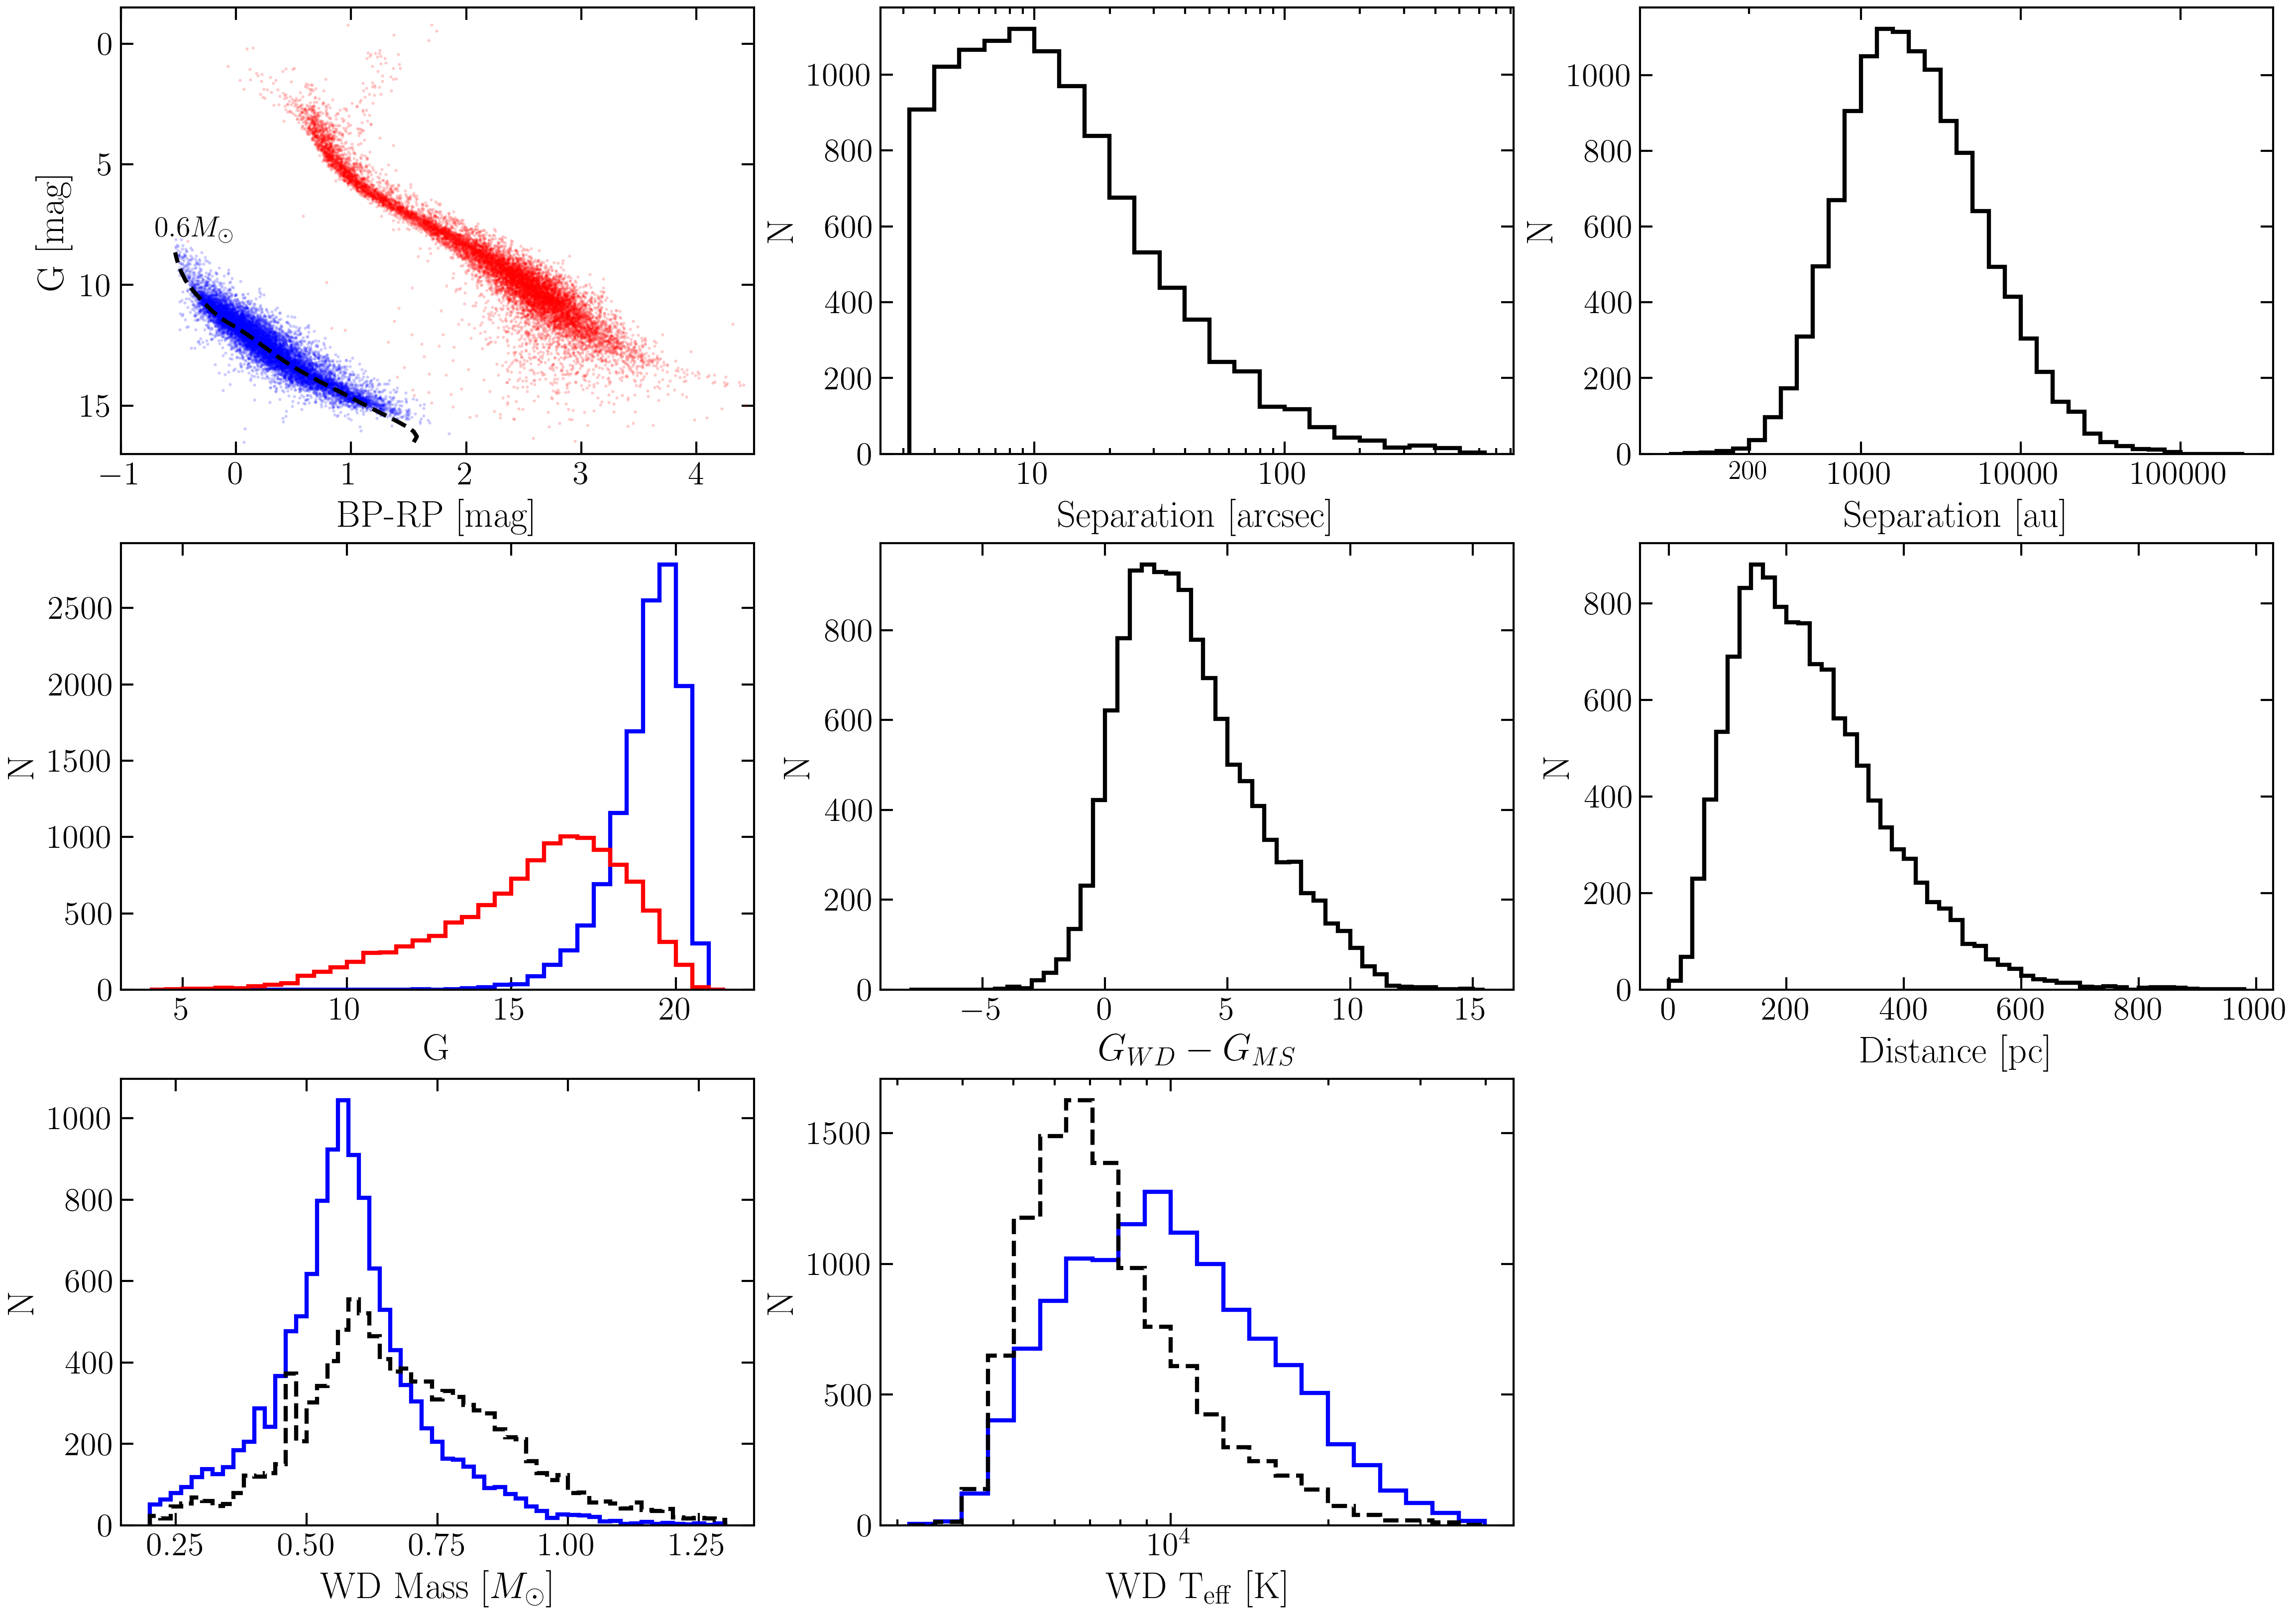
\includegraphics[width=\columnwidth]{sample_summary.png}
    \caption{A summary of the wide WD+MS sample used in this work. The top left panel shows a CMD with the white dwarfs shown in blue and MS components in red. The top middle and top right panel show the separation distribution of the sample in angular and physical units. Magnitude distributions of the MS (red) and white dwarfs (blue) are shown in the middle left panel with the magnitude difference of the binaries is shown in the middle panel. A histogram of the distances of each system (determined through the weighted parallax of the system) is shown in the middle right panel. Finally, the derived white dwarf masses and effective temperatures are shown in the bottom panels. For the bottom panels, an additional cut has been applied to remove white dwarfs with temperatures near the edge of our model grid ($3200 < T_{\text{eff}} < 38{,}000$~K). }
    \label{fig:sample_summary}
\end{figure}

\subsection{White Dwarf Spectral Types}

As found in \cite{2024arXiv240502423H}, it is important to have spectral type information when determining the most reliable white dwarf total ages. In this work, we gather spectral types from a variety of sources in the literature as well as spectral types determined through Gaia XP spectra \citep{2024ANA...682A...5V}. We find 6460 white dwarfs in the sample have spectral types determined in the literature with 5267 being determined solely through their Gaia XP spectra (see Table~\ref{tab:spec_types}).

\begin{deluxetable}{ccc}
\centering
\tabletypesize{\normalsize}
\tablewidth{0.75\textwidth}
\tablecolumns{3}
\tablecaption{Spectral Types in the WD+MS Sample \label{tab:spec_types}
}
\tablehead{
        \colhead{Spectral Type} &
         \colhead{$N_{tot}$}  &
         \colhead{$N_{Gaia XP}$}
        }
\startdata
DA & 5233 & 4417\\
DB & 394 & 316\\
DC & 600 & 433\\
DQ & 65 & 33\\
DZ & 79 & 60\\
Other & 89 & 0\\
\enddata
\tablecomments{The spectral types in this work are gathered from \cite{2024ANA...682A...5V} and the Montreal White Dwarf Database as well as the following sources: \cite{1999ApJS..121....1M,2004MNRAS.349.1397C,2006ApJS..167...40E,2009ANA...505..441K,2011ApJ...737...28B,2011ApJ...743..138G,2011ApJ...741...64K,2011AJ....141...96L,2011ApJ...730..128T,2012MNRAS.426.1235V,2013MNRAS.429.2143C,2013ApJS..204....5K,2013MNRAS.431..240O,2015MNRAS.448.2260G,2015MNRAS.446.4078K,2015MNRAS.453.1879K,2016MNRAS.455.3413K,2017MNRAS.465.2849T,2019ApJ...885...74C,2019MNRAS.482.4570G,2019MNRAS.486.2169K,2020ApJ...901...93B,2020ANA...635A.193G,2021MNRAS.508.3877G,2022ApJ...934...36B,2023MNRAS.519.4529C,2023MNRAS.520.6111H,2024MNRAS.527.8687O}}
\end{deluxetable}

\subsection{Metallicities}

The metallicities of the MS components in this work are taken from three sources; DR3 of the GALactic Archaeology with HERMES survey (GALAH, \citealt{2015MNRAS.449.2604D, 2021MNRAS.506..150B}), DR17 of the Apache Point Observatory Galactic Evolution Experiment (APOGEE, \citealt{2017AJ....154...94M, 2022ApJS..259...35A}), and DR5 of the Large Sky Area Multi-Object Fiber Spectroscopic Telescope (LAMOST, \citealt{2012RAA....12.1197C, 2019ApJ...881....7L}). Specifically, we compile $\left[\mathrm{Fe/H}\right]$ from all sources, $\left[\mathrm{Li/Fe}\right]$ from GALAH, and $\left[\mathrm{\alpha/Fe}\right]$ and $\left[\mathrm{C/Fe}\right]$ from GALAH and APOGEE.

APOGEE and GALAH provide quality flags for the individual abundance measurements. To ensure the quality of the metallicities in this work, we remove abundances that have any raised flags in APOGEE and remove abundances with flags above one for GALAH. Abundances flagged with a value of one in GALAH denote upper limits, which are still valuable in the analysis in this section. With these cuts, 582 systems have measurements of $\left[\mathrm{Fe/H}\right]$, 69 systems (26 upper limits) have a measurement of $\left[\mathrm{Li/Fe}\right]$, 332 systems have a measurement of $\left[\mathrm{\alpha/Fe}\right]$, and 147 systems (19 upper limits) have a measurement of $\left[\mathrm{C/Fe}\right]$.

\section{White Dwarf Age Determinations} \label{sec:age_determ_WDMS}
The white dwarf total ages are determined through fitting their spectral energy distributions (SEDs) using optical photometry from Gaia, the Panoramic Survey Telescope and Rapid Response System (PanSTARRS), the Sloan Digital Sky Survey (SDSS), and the SkyMapper Southern Sky Survey.

\subsection{Fitting Routine}\label{sec:fitting}
I follow the same methods outlined in Chapters \ref{sec:chap2} and \ref{sec:chap3}. To summarize, we convert model white dwarf spectra to synthetic fluxes by using the sensitivity of each bandpass and the appropriate AB magnitude zeropoints. Weuse the DA models of \cite{2010MmSAI..81..921K} for all DA, DAH, and DAZ white dwarfs, the mixed H/He atmospheres from \cite{2021MNRAS.501.5274C} with H/He of $10^{-5}$ for all DBA white dwarfs and DC and DZ white dwarfs with temperatures between 5500~K and 11,000K, and the pure He models from \cite{2021MNRAS.501.5274C} for all DB, DBZ, and DQ white dwarfs, and DC and DZ white dwarfs with temperatures greater than 11,000~K. For DC and DZ white dwarfs with temperatures less than 5500~K, the same pure H models as the DAs are used.

The observed magnitudes are also converted to absolute fluxes at 10 pc using AB zeropoints and the weighted mean parallax of the binary from Gaia. For SDSS $u$ and $z$, the magnitudes are shifted $0.04$ and $0.02$ mag, respectively, to account for the shift relative to the AB mag system \citep{2004AJ....128..502A}. The weighted mean parallax is on average five times more precise than the individual white dwarf parallax which in turn allows for a more precise age determination. Comparing to the Gaia EDR3 catalog of white dwarfs \citep{2021MNRAS.508.3877G}, we find the mass errors are improved by a factor of 2.5 on average (see Figure~\ref{fig:errors}). In Chapter~\ref{sec:chap2}, the observed fluxes are de-reddened using a 2D extinction map with a linear distance parameterization \citep{2011ApJ...737..103S}. In this work, the observed fluxes are de-reddened using extinction values from \cite{2021MNRAS.508.3877G}, which are obtained using an early version of the 3D extinction maps from \cite{vergley2022}. These observed de-reddened fluxes are related to the model synthetic fluxes through the radius of the white dwarf.

\begin{figure}
    \centering
    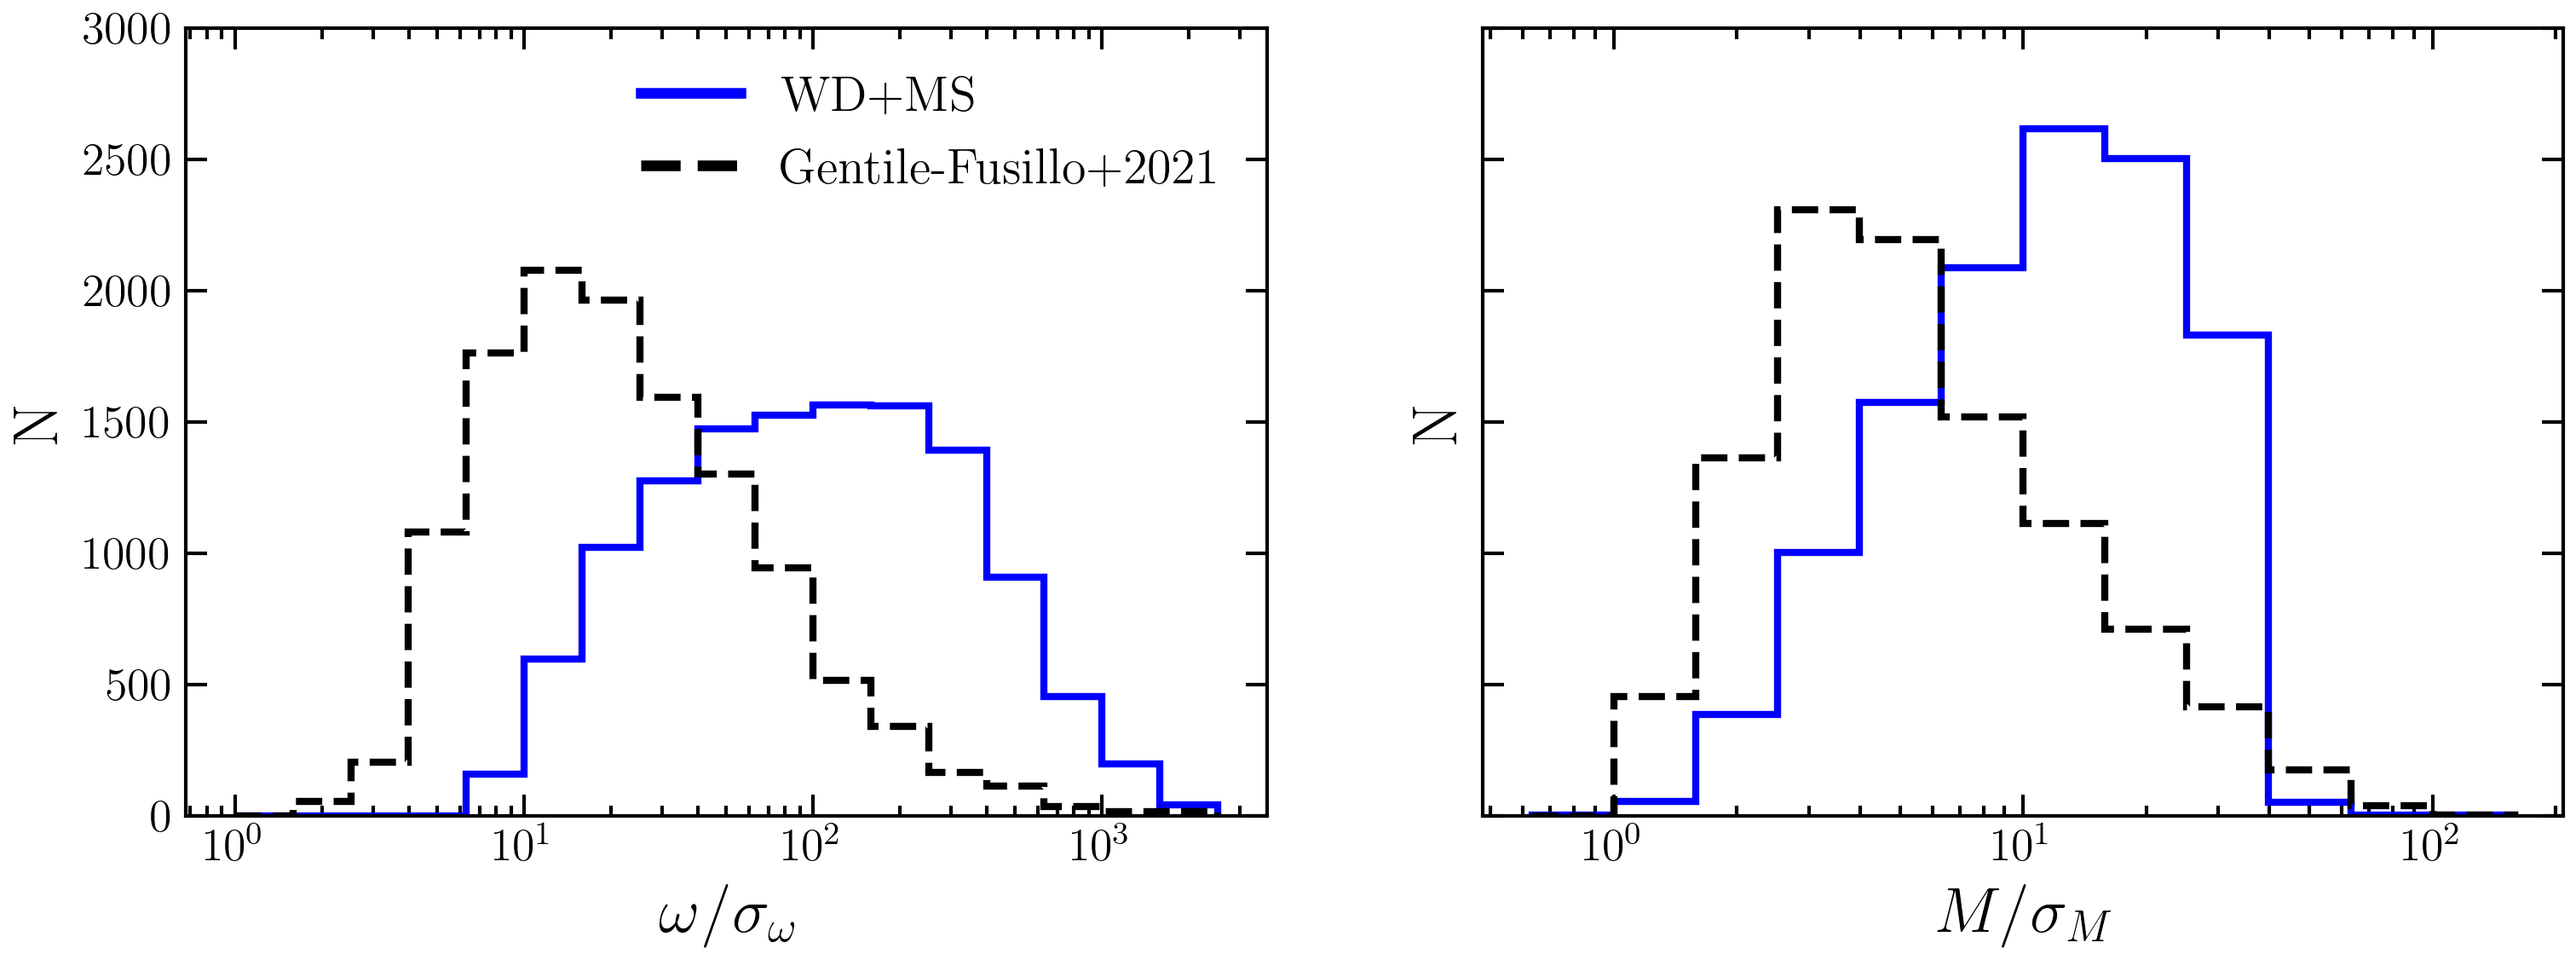
\includegraphics[width=\columnwidth]{errors_histograms.png}
    \caption{Histograms of the parallax over error and mass over error for the WD+MS sample (blue) and the EDR3 white dwarf catalog of \cite{2021MNRAS.508.3877G} (dashed black). The parallax errors are improved by a factor of 5 on average and the mass errors are improved by a factor of 2.5 on average.}
    \label{fig:errors}
\end{figure}

I use a Markov Chain Monte Carlo approach and make use of the python package \texttt{emcee} \citep{2013PASP..125..306F} to get best-fit temperatures and radii, which are represented by the 50$^\mathrm{th}$ percentiles of the MCMC posterior distributions. These are converted to surface gravities, masses, and cooling ages using the cooling models from \cite{2020ApJ...901...93B}. We use the thick H layer cooling models for the hydrogen fits, the thin H layer cooling models for the mixed atmosphere fits, and the pure He cooling models for the He atmosphere fits. We use flat priors for the temperatures and surface gravities that cover the full range of the models. A lower limit on the magnitude uncertainties of 0.03 mag is set to account for systematics in the conversion of magnitudes to average fluxes. We also impose a lower uncertainty on the surface gravities of 0.03 dex and a lower uncertainty of 1.2\% on the effective temperatures to account for any unknown systematics in the models (e.g., \citealt{2005ApJS..156...47L}).

\subsection{Photometric Cleaning}
Just as in Chapters~\ref{sec:chap2} and \ref{sec:chap3}, we remove photometry that is flagged in SDSS, PanSTARRS, and SkyMapper. We remove photometry from SDSS with \texttt{EDGE}, \texttt{PEAKCENTER}, \texttt{SATUR}, and \texttt{NOTCHECKED} flags. We only use photometry from PanSTARRS with rank detections of 0 or 1. We also remove any photometry from SkyMapper that has any raised flags.

There is often a large luminosity contrast between the white dwarf and main-sequence star in the binary, therefore an added measure of cleaning of the photometry is needed to obtain reliable parameters. To alleviate this problem, we systematically remove photometry that is not consistent with the Gaia fluxes. To do this, we run our fitting routine described in Section \ref{sec:fitting}. Then, we fit a line to the residuals of the resulting SED fit to account for an incorrect temperature estimate. We compare the residuals of this linear fit to the largest absolute percent deviation between Gaia  $\mathrm{G, G_{BP},\ and\ G_{RP}}$. Any photometric bands that are more than $3\sigma$ away from this absolute percent deviation are removed, where $\sigma$ is the uncertainty for the individual photometric band. A new linear fit to the SED residuals is performed with these bands removed. Then, a new comparison to the largest absolute percent deviation of the Gaia bands is performed, including the previously removed bands. This iterative process continues until a consistent list of photometric bands are removed, and a final SED fit is performed. SDSS $u$-band is not subjected to this stage of photometric cleaning since it can be a strong indicator of whether the white dwarf is a DA or non-DA due to the presence of the Balmer jump in DA WDs. The larger residual of SDSS $u$ can be indicative of a non-DA and not because the photometry is suspect (e.g. \citealt{2019ApJ...876...67B}). 

There are 1845 white dwarfs refit through this process. The refits result in absolute mass changes of 0.1~\msun\ on average which results in significant changes in the derived total ages. The change in mass tends to push the white dwarf masses to higher values (0.02~\msun\ on average) which is encouraging given we are removing apparent blended photometry in the red portion of the SED from the MS companion. This results in slight changes in temperature determinations (usually the new fits return hotter temperatures), which requires smaller radii and higher masses. We also find the reduced $\chi^{2}$ values decrease for the majority of the redone fits with an average reduction by a factor of 2.5.

\subsection{Progenitor Lifetimes}
To get the progenitor lifetimes of the white dwarfs, we use the same initial-final mass relation (IFMR) outlined in Chapter~\ref{sec:chap2} which uses a theoretically motivated shape to the IFMR from \citet{2016ApJ...823...46F}, fit to white dwarfs in solar metallicity clusters \citep{2015ApJ...807...90C,2016ApJ...818...84C}, in conjunction with the stellar evolutionary tracks from Modules for Experiments in Stellar Astrophysics (MESA, \citealt{2011ApJS..192....3P}, \citealt{2013ApJS..208....4P}, \citealt{2015ApJS..220...15P}). The errors on these values are determined by using the $1\sigma$ uncertainties on the WD mass to determine an upper and lower MS mass. The difference between the central value and the upper and lower MS mass are quoted as upper and lower errors, respectively. The same process is carried out for the progenitor lifetimes as well.

\section{Results}\label{sec:chap4_results}

\subsection{Age-Metallicity Relation}\label{sec:metal}

Here, we investigate the relation between the MS star's metallicity, specifically $\left[\mathrm{Fe/H}\right]$, and the white dwarf component's total age. To ensure reliable ages and metallicities, we perform a few quality cuts. We restrict the sample to white dwarfs with masses greater than 0.63\msun\ given the results in Chapter~\ref{sec:chap2}. We also restrict the sample to white dwarfs with effective temperatures greater than 3200~K to avoid edge effects of the MCMC. After these cuts, the sample size becomes 198 systems with measured values of $\left[\mathrm{Fe/H}\right]$ and system age.

Figure~\ref{fig:AMR_scatter} shows how metallicity changes as a function of the white dwarf's total age. We split the sample based on the source of the metallicity to avoid any systematic differences between the three catalogs introduced through differing data reduction and wavelength coverage. A linear fit is shown in each panel to show if any significant trends are seen. We do not find a significant trend in the GALAH and LAMOST samples but do find the expected decrease in age as a function of metallicity in the APOGEE data with lower metallicity stars tending to be older on average. Figure~\ref{fig:AMR_medians} shows this trend in a different way. Plotted is a running average of the white dwarf total age as a function of the MS star's metallicity. The bins for the APOGEE and LAMOST samples run from $-0.6$~dex to $0.4$~dex in steps of $0.05$~dex. We choose the bin size to be $0.1$~dex to increase the number of systems per bin, which does lead to some overlap between neighbouring bins. Due to the smaller sample size of the GALAH sample, the bins run from $-0.6$~dex to $0.4$~dex in steps of $0.1$~dex with a bin size of $0.2$~dex. Only bins with three or more systems are plotted. The maximum number of systems per bin is 7, 15, and 27 for GALAH, APOGEE, and LAMOST, respectively. The standard deviation in the total ages for each metallicity bin is shown as the shaded regions in each panel. The median total age in a given bin decreases with metallicity for the APOGEE sample, but the scatter about that median shows that the correlation is weak.

\begin{figure}
    \centering
    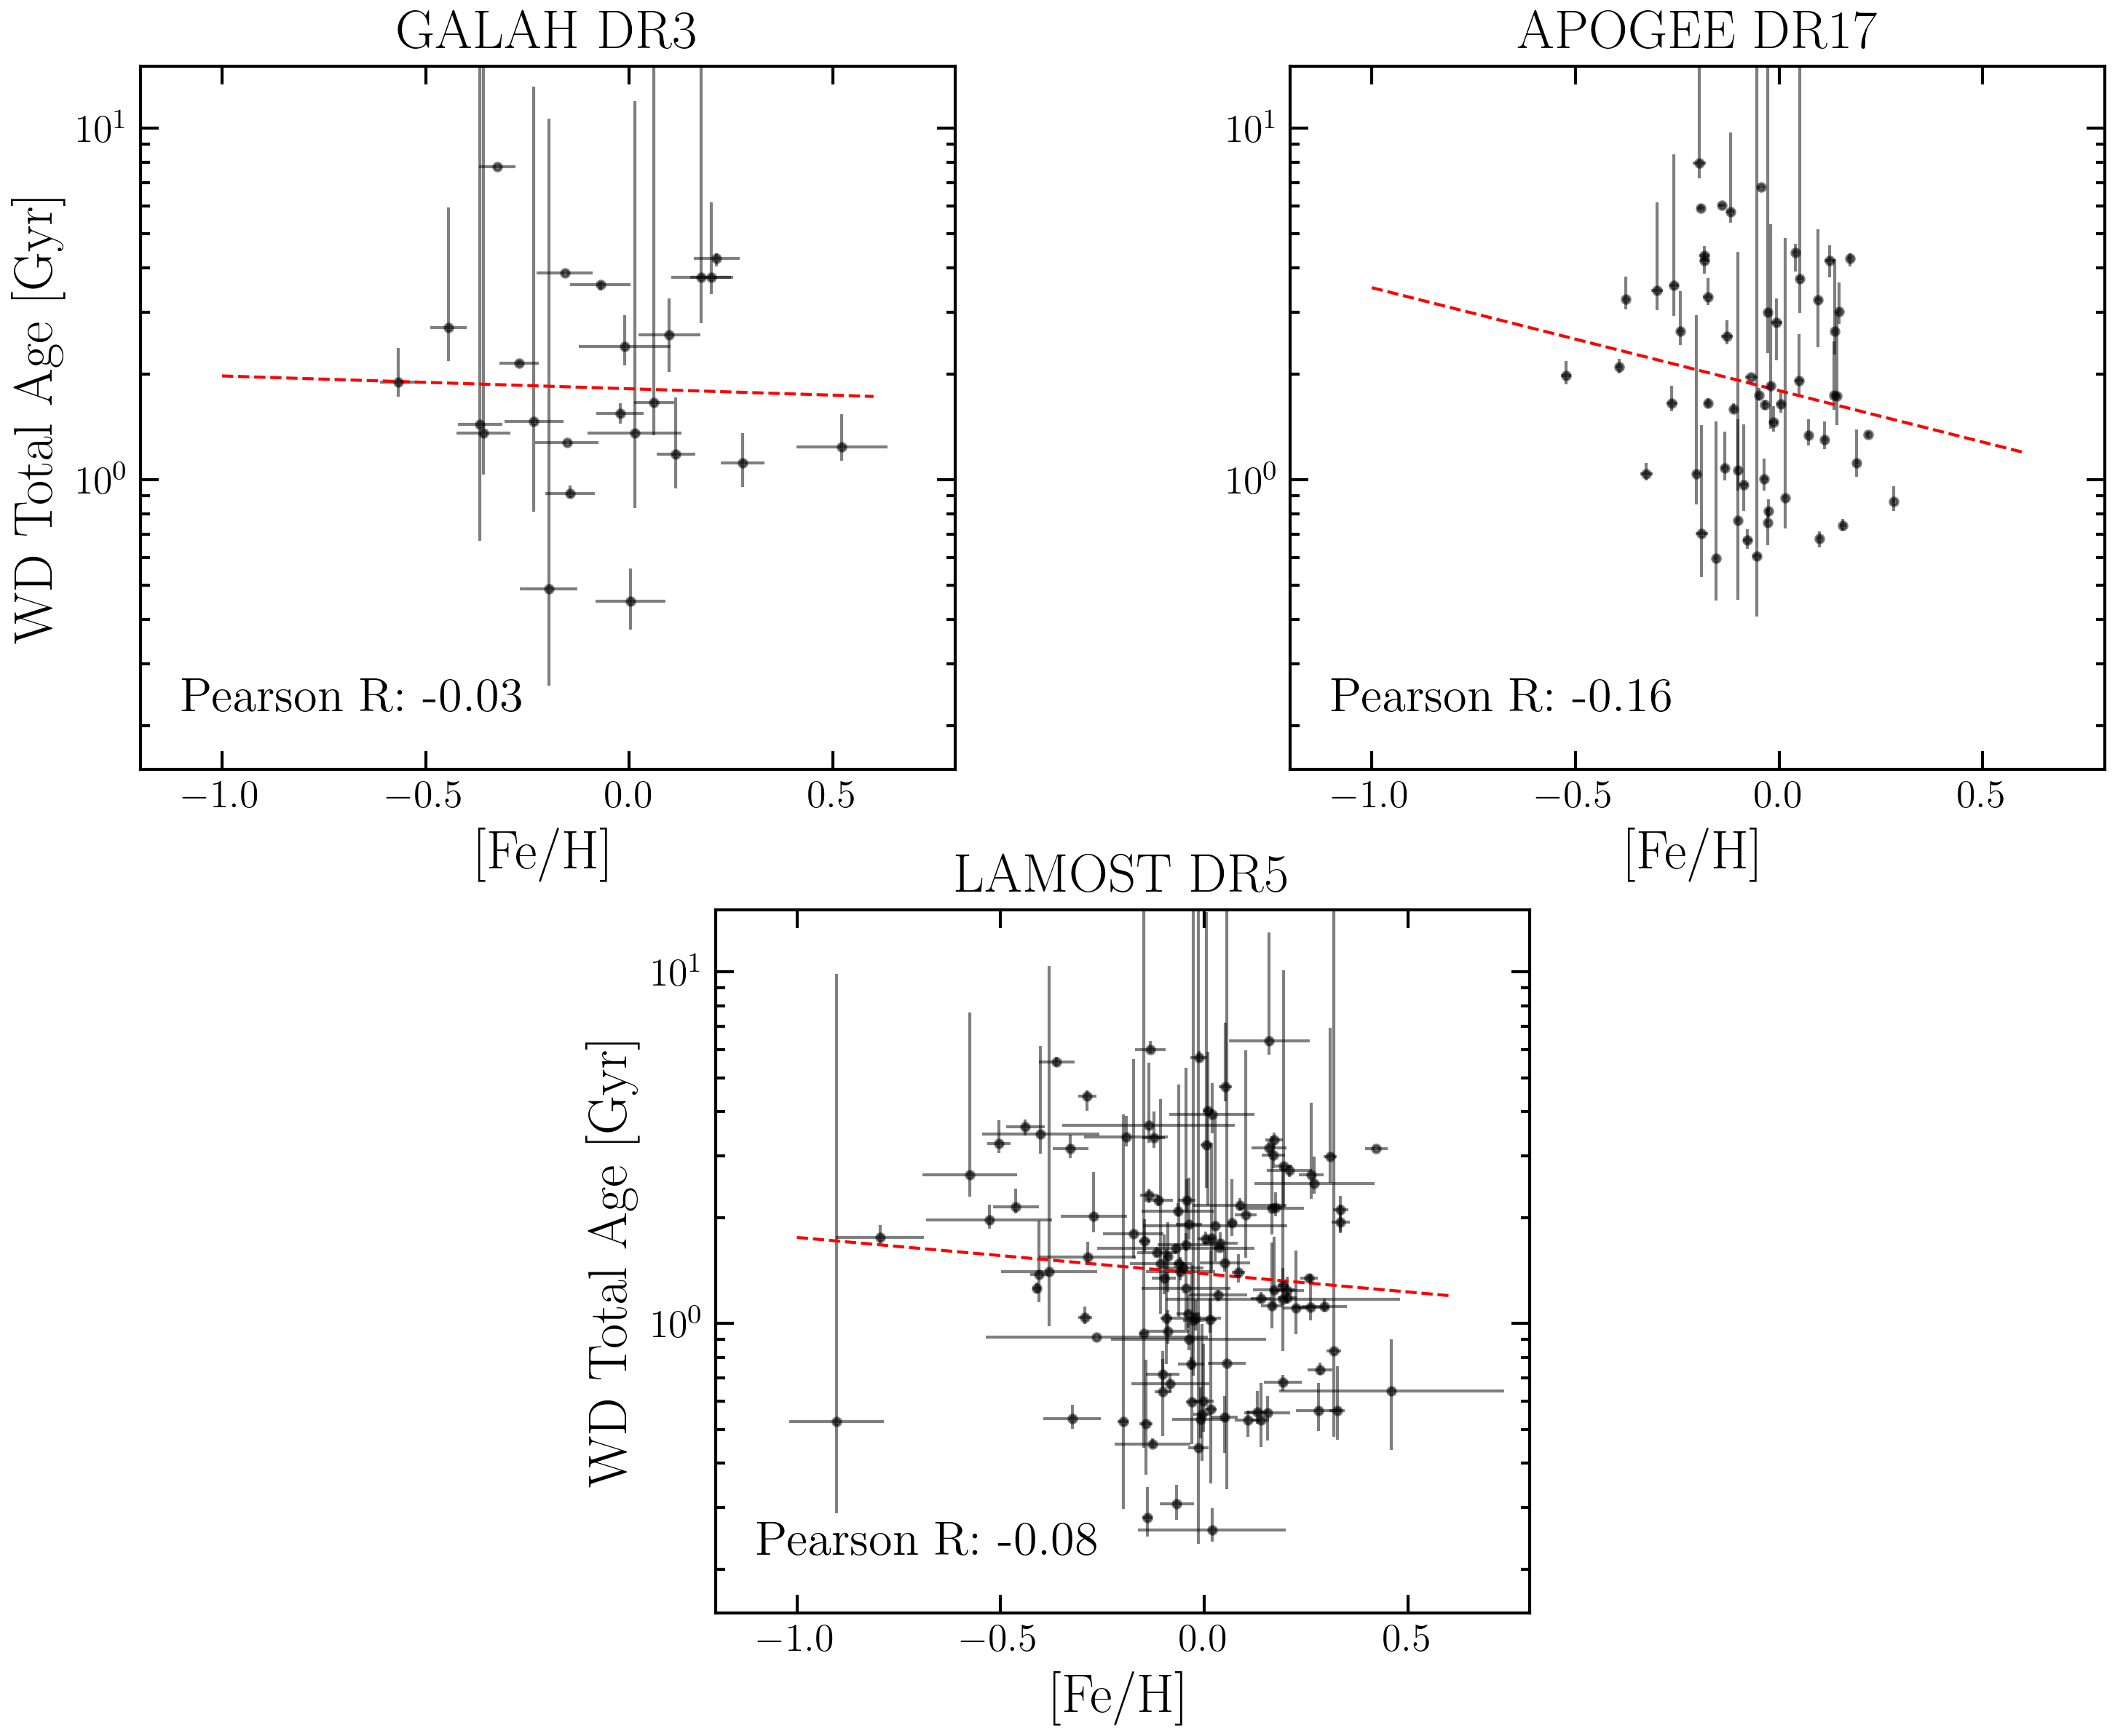
\includegraphics[width=\columnwidth]{AMR_scatter.png}
    \caption{White dwarf total age as a function of metallicity. Each panel displays a linear fit to the data in red to show any trends present. A Pearson correlation coefficient is also provided in each panel to denote the strength of the correlation. There are no significant trends seen in the GALAH and LAMOST samples but a weak trend of decreasing age with increasing metallicity is seen in the APOGEE sample.}
    \label{fig:AMR_scatter}
\end{figure}

\begin{figure}
    \centering
    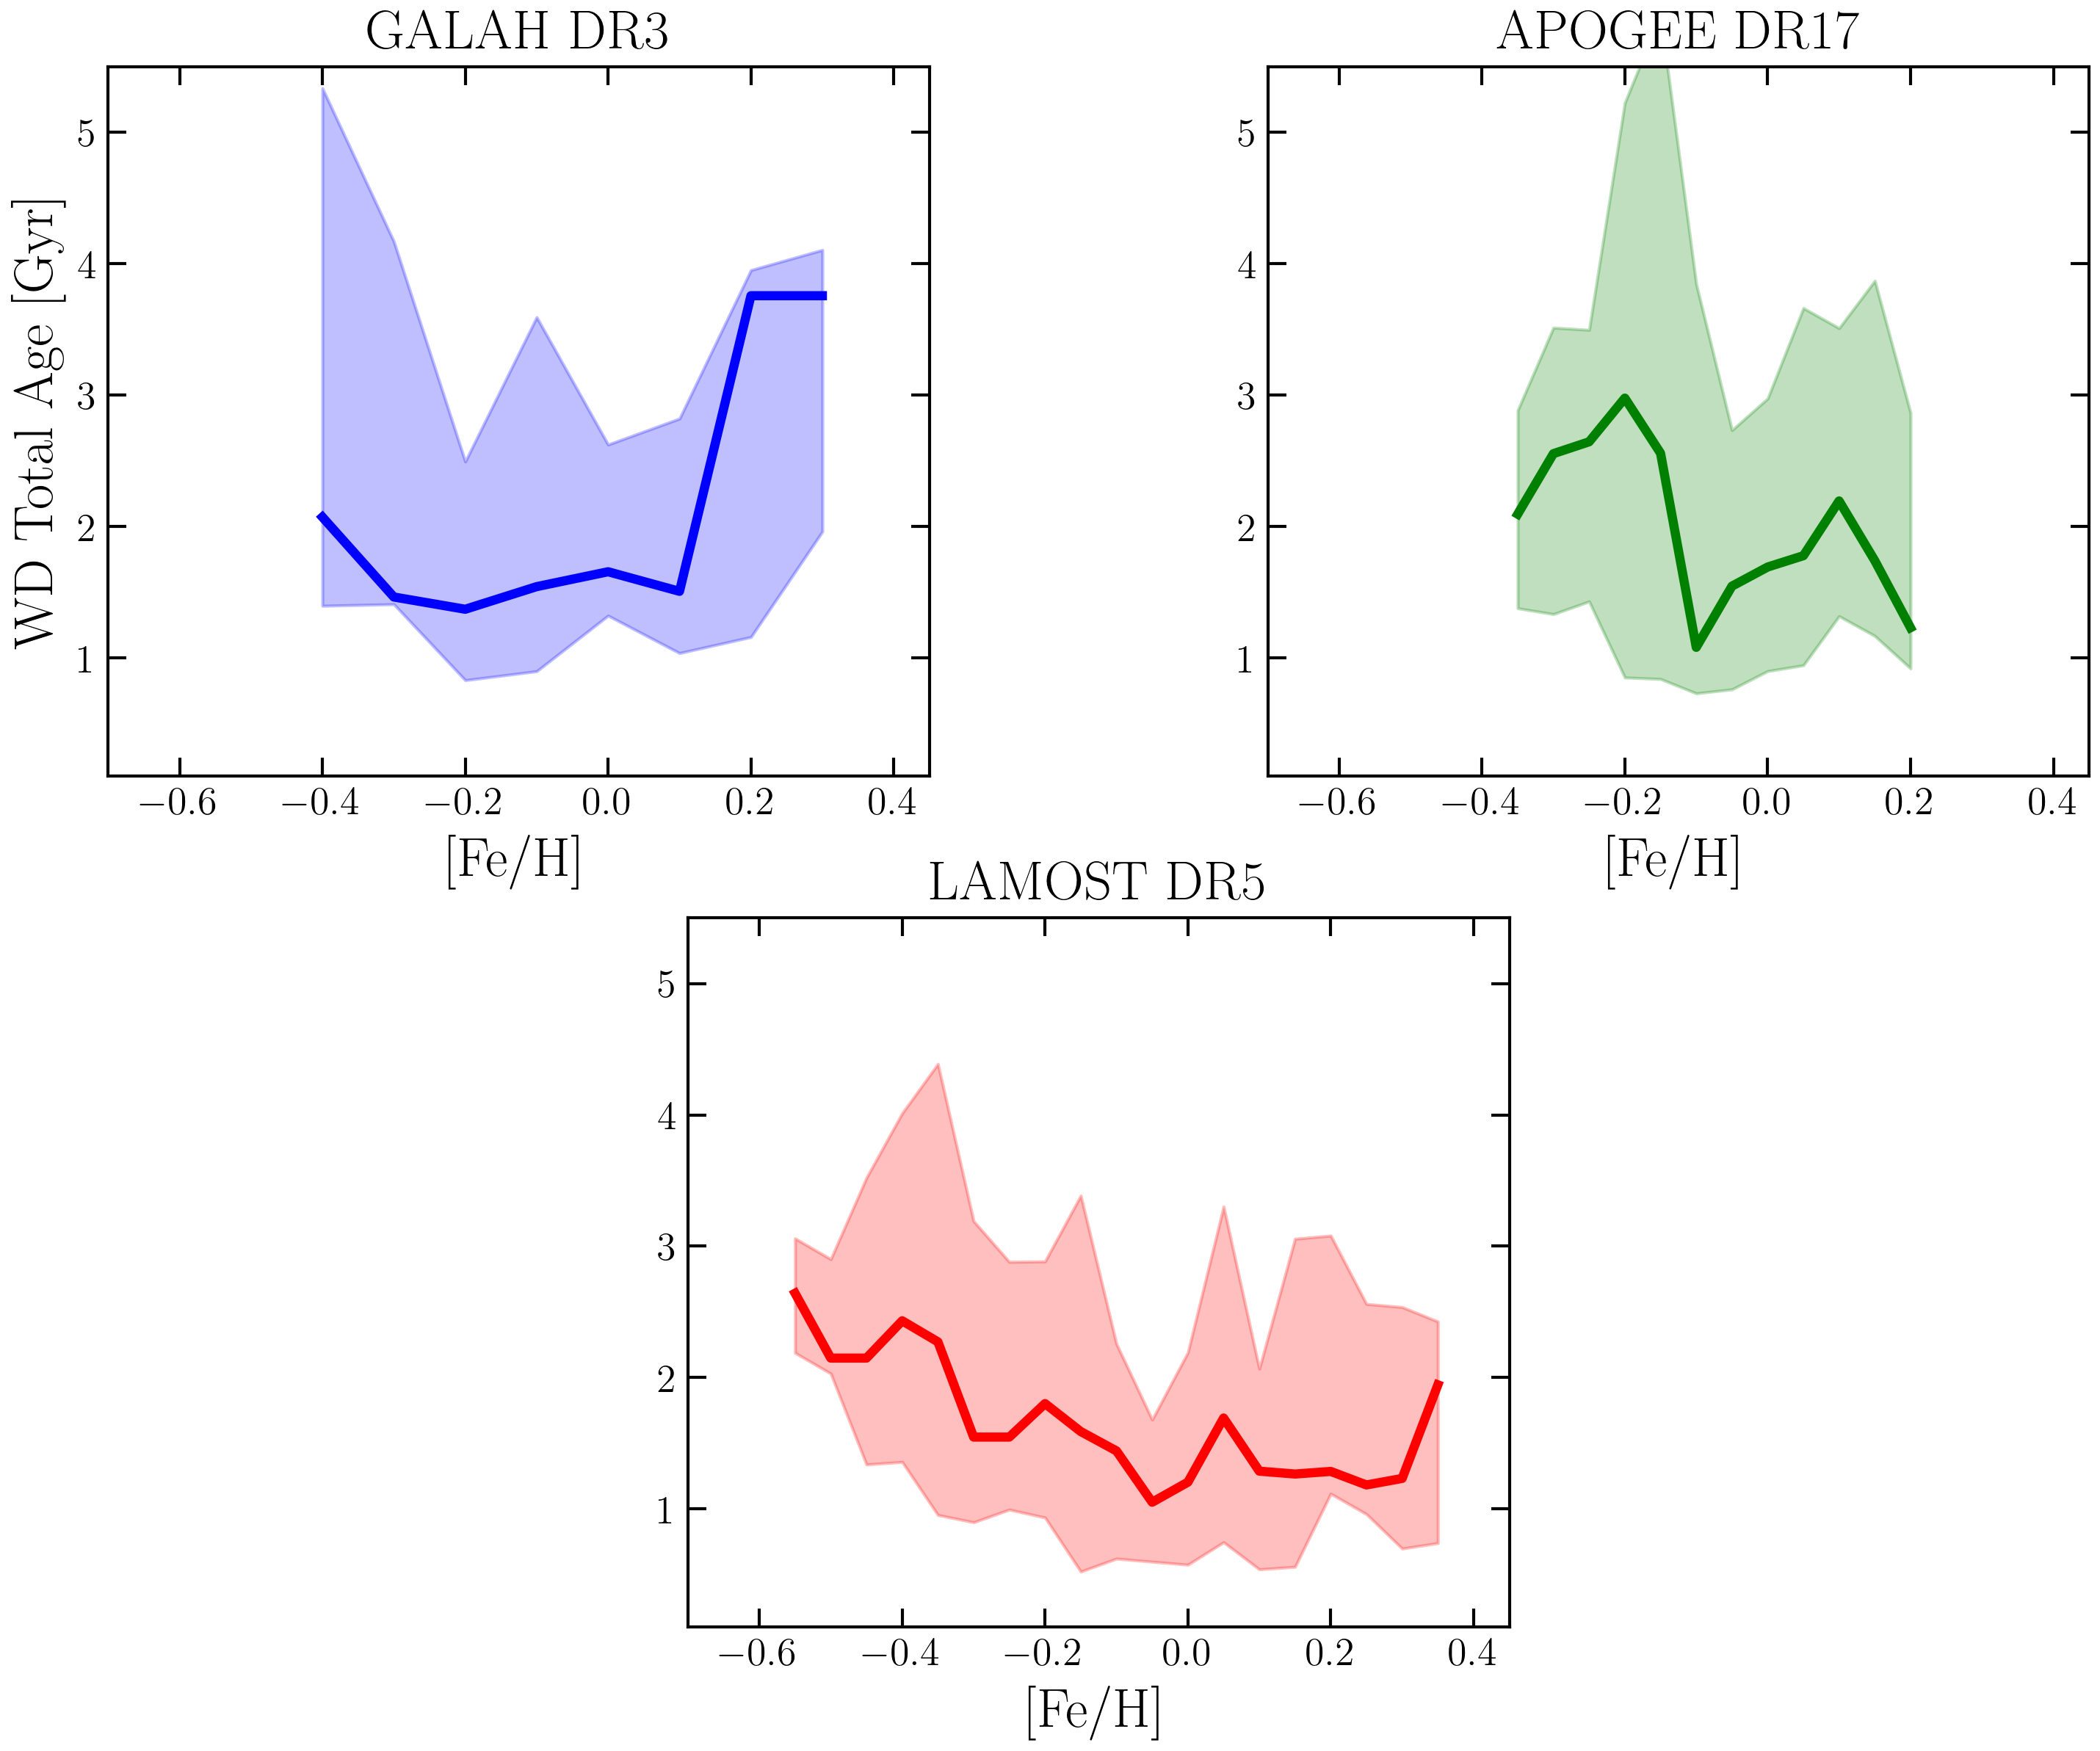
\includegraphics[width=\columnwidth]{AMR_medians.png}
    \caption{White dwarf total age as a function of metallicity. The solid line represents the median value of a metallicity bin with a width of 0.1 dex while the shaded region represents the 16th to 84th percentile.}
    \label{fig:AMR_medians}
\end{figure}

The GALAH and LAMOST samples do not show the expected trend between age and metallicity, which may be indicative of problems with the white dwarf total ages. If white dwarf total ages are accurate and reliable, one would expect the total ages to follow the trend seen in the APOGEE data. A possible explanation is that the APOGEE data has more precisely measured metallicities. In this sample, the APOGEE metallicities have an average uncertainty (0.01~dex) three times smaller than the LAMOST metallicity uncertainties (0.03 dex) and six times smaller than the GALAH metallicity uncertainties (0.06 dex). In terms of total age uncertainties, the GALAH sample has large relative total age errors compared to the other two samples. The LAMOST and APOGEE samples have average relative age uncertainties of order 10\% while the GALAH sample has an average relative total age error of order 25\%, due to the GALAH sample being comprised of fainter white dwarfs on average when compared to the APOGEE and LAMOST samples. It should also be noted that the GALAH sample has 24 systems while the APOGEE sample has 57 systems. This makes the results from the GALAH sample not as statistically significant as the APOGEE sample. The LAMOST sample is the largest, with 115 systems. 

When determining the progenitor lifetimes for the white dwarfs, solar metallicity stellar evolutionary tracks were used as well as an IFMR calibrated with solar metallicity clusters. Metallicity is known to play an important role in stellar lifetimes and the IFMR. Higher metallicity stars produce less massive white dwarfs due to increased mass-loss rates from higher opacities and subsequently, have longer lifetimes \citep{2015MNRAS.450.3708R}. We investigate whether the use of the appropriate metallicity stellar evolutionary grids affects the findings in this section. To test this, we take the same stellar evolutionary grids from MESA with zero-rotation but with metallicities of $\left[\mathrm{Fe/H}\right] = -0.5$, $-0.25$, and $0.25$. As can be seen in Figure~\ref{fig:age_vs_metallicity}, stars with higher metallicities have longer progenitor lifetimes which produces the opposite of the desired effect by making high metallicity systems even older. This effect is of order 10-20\% on the estimated progenitor lifetime for the majority of the sample but produces a smaller change in the actual total age on the order of a few percent (see right panel of Figure~\ref{fig:age_vs_metallicity}) due to the cooling age being the dominant age component for the majority of the sample.
 
 \begin{figure}
     \centering
     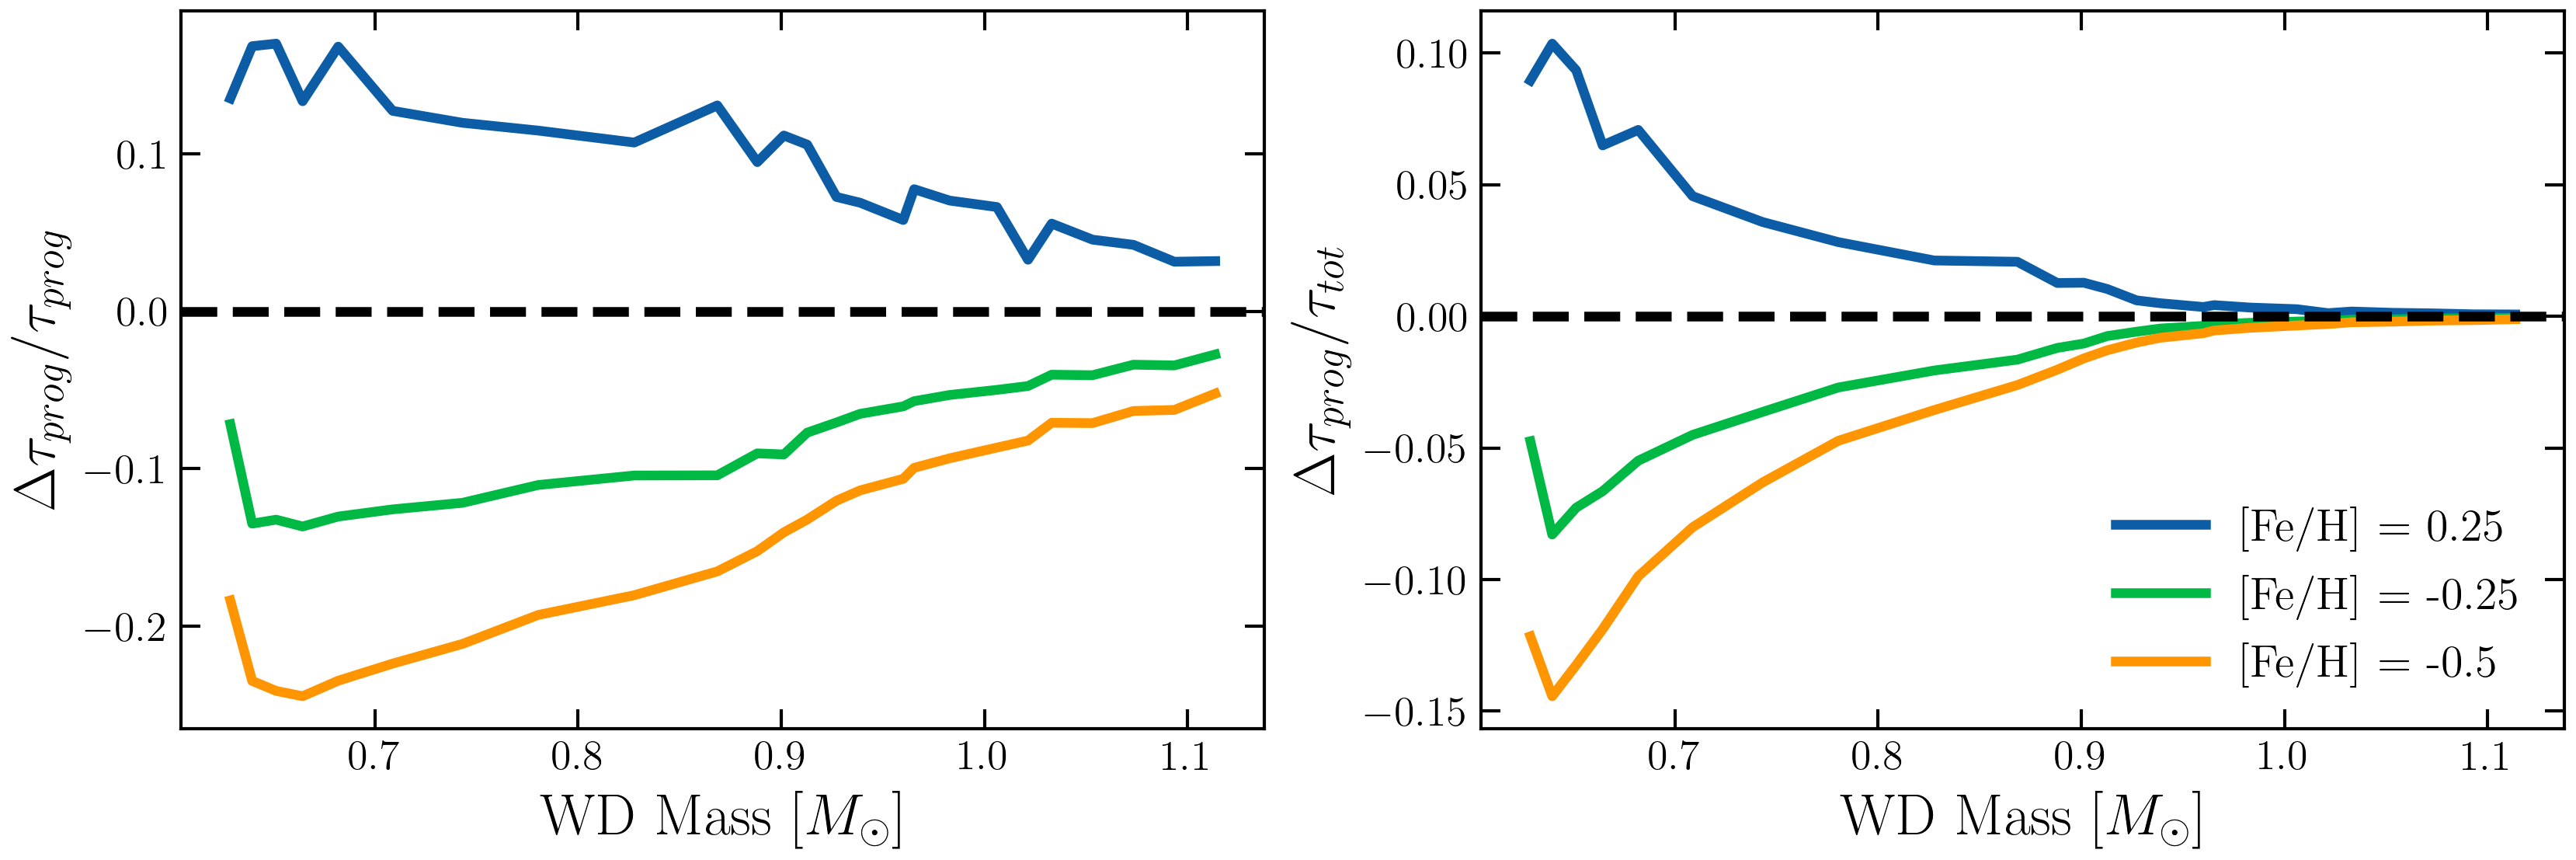
\includegraphics[width=\columnwidth]{age_vs_metallicity.png}
     \caption{The relative difference between ages derived from stellar grids of solar metallicity and other selected metallicities as a function of white dwarf mass. The left panel shows the change in progenitor lifetime, while the right panel shows the equivalent change in total age for a 10,000~K white dwarf. For the lowest mass white dwarfs in the sample, this change is of order 10-20\% on the progenitor lifetime and on the order of a few percent in terms of total age.}
     \label{fig:age_vs_metallicity}
 \end{figure}

It is difficult to account for the dependence of the IFMR on the progenitor metallicity. It is expected to cause higher-metallicity stars to produce lower-mass white dwarfs. This means for the high metallicity systems in the sample, we are underestimating the ZAMS mass and thus over-estimating the ages. This will act against the effect explored in the previous paragraph. Some work has been done to determine the change in the IFMR for changing metallicities. \cite{2015MNRAS.450.3708R} developed theoretical IFMRs of varying metallicities and found progenitor lifetimes can change by large fractions over a small metallicity window of few hundredths of a dex. \cite{2024MNRAS.527.3602C} found a more modest effect of metallicity on the IFMR with variations in the estimated initial ZAMS mass on the order of 0.1 \msun. This can still produce significant progenitor lifetime differences for the lowest mass white dwarfs where the progenitor lifetimes have large changes as a function of ZAMS mass.

The lack of correlation between age and metallicity among WD+MS binaries was previously observed by \cite{2021MNRAS.505.3165R}. In their work, they used a sample WD+MS binaries from SDSS in conjunction with metallicity measurements derived from K-band magnitudes as well as a sample of WD+MS binaries taken from \cite{2016MNRAS.458.3808R}. Their results, in conjunction with those here, provide evidence of no correlation between metallicity and age in the solar neighbourhood, with the important caveat that that the ages in this sample are generally $<5$~Gyr.

\subsection{Age vs. Lithium Abundance}

Lithium abundance is expected and observed to correlate strongly with stellar age. This has been investigated extensively in solar analogues \citep[e.g.,][]{2016A&A...587A.100C, 2023MNRAS.522.3217M} showing lithium is depleted as a star ages. Recent work uses the equivalent width of lithium to reproduce ages for low-mass stars in open clusters at an effective rate \citep{2023MNRAS.523..802J}. Using the data gathered from GALAH, we investigate if similar trends can be seen in our data set. We restrict the sample to white dwarfs with temperatures greater than 3200~K to avoid edge effects of the MCMC fits and white dwarf ages with measured ages less than 12~Gyr. This results in sample of eight systems with measured white dwarf ages and measured Li abundances.

Lithium abundances are conventionally represented by $A(Li) = \log{(N_{Li}/N_H)} + 12$. We convert the [Li/Fe] into $A(Li)$ following \cite{2022A&A...668A.181B} by the following formula:
\begin{equation}
    A(Li) = [Li/Fe] + [Fe/H] + A(Li)_\odot
\end{equation}
where $A(Li)_\odot$ is the solar lithium abundance = 0.96 dex \citep{2021MNRAS.500.2159W}.

Figure~\ref{fig:lithium} shows how lithium abundances change as a function of age in our sample. Figure~\ref{fig:lithium} also shows the temperature of the MS star as a proxy for mass. Lithium abundances have been shown to also depend on the mass of the star as well as its age \citep[e.g.][]{2015A&A...579A.122A} and the expected trend is seen in our sample. We find lithium abundances do decrease as a function of age for specific temperature bins. The high ($>5750$~K) and low ($<5100$~K) temperature bins show the expected decrease as a function of age but the middle temperature bin is a little less clear. These bins separate the already small data set into even smaller data sets, which makes any conclusions susceptible to outliers, but there are no obvious problems that would raise concern over the white dwarf age estimates. 

\begin{figure}
    \centering
    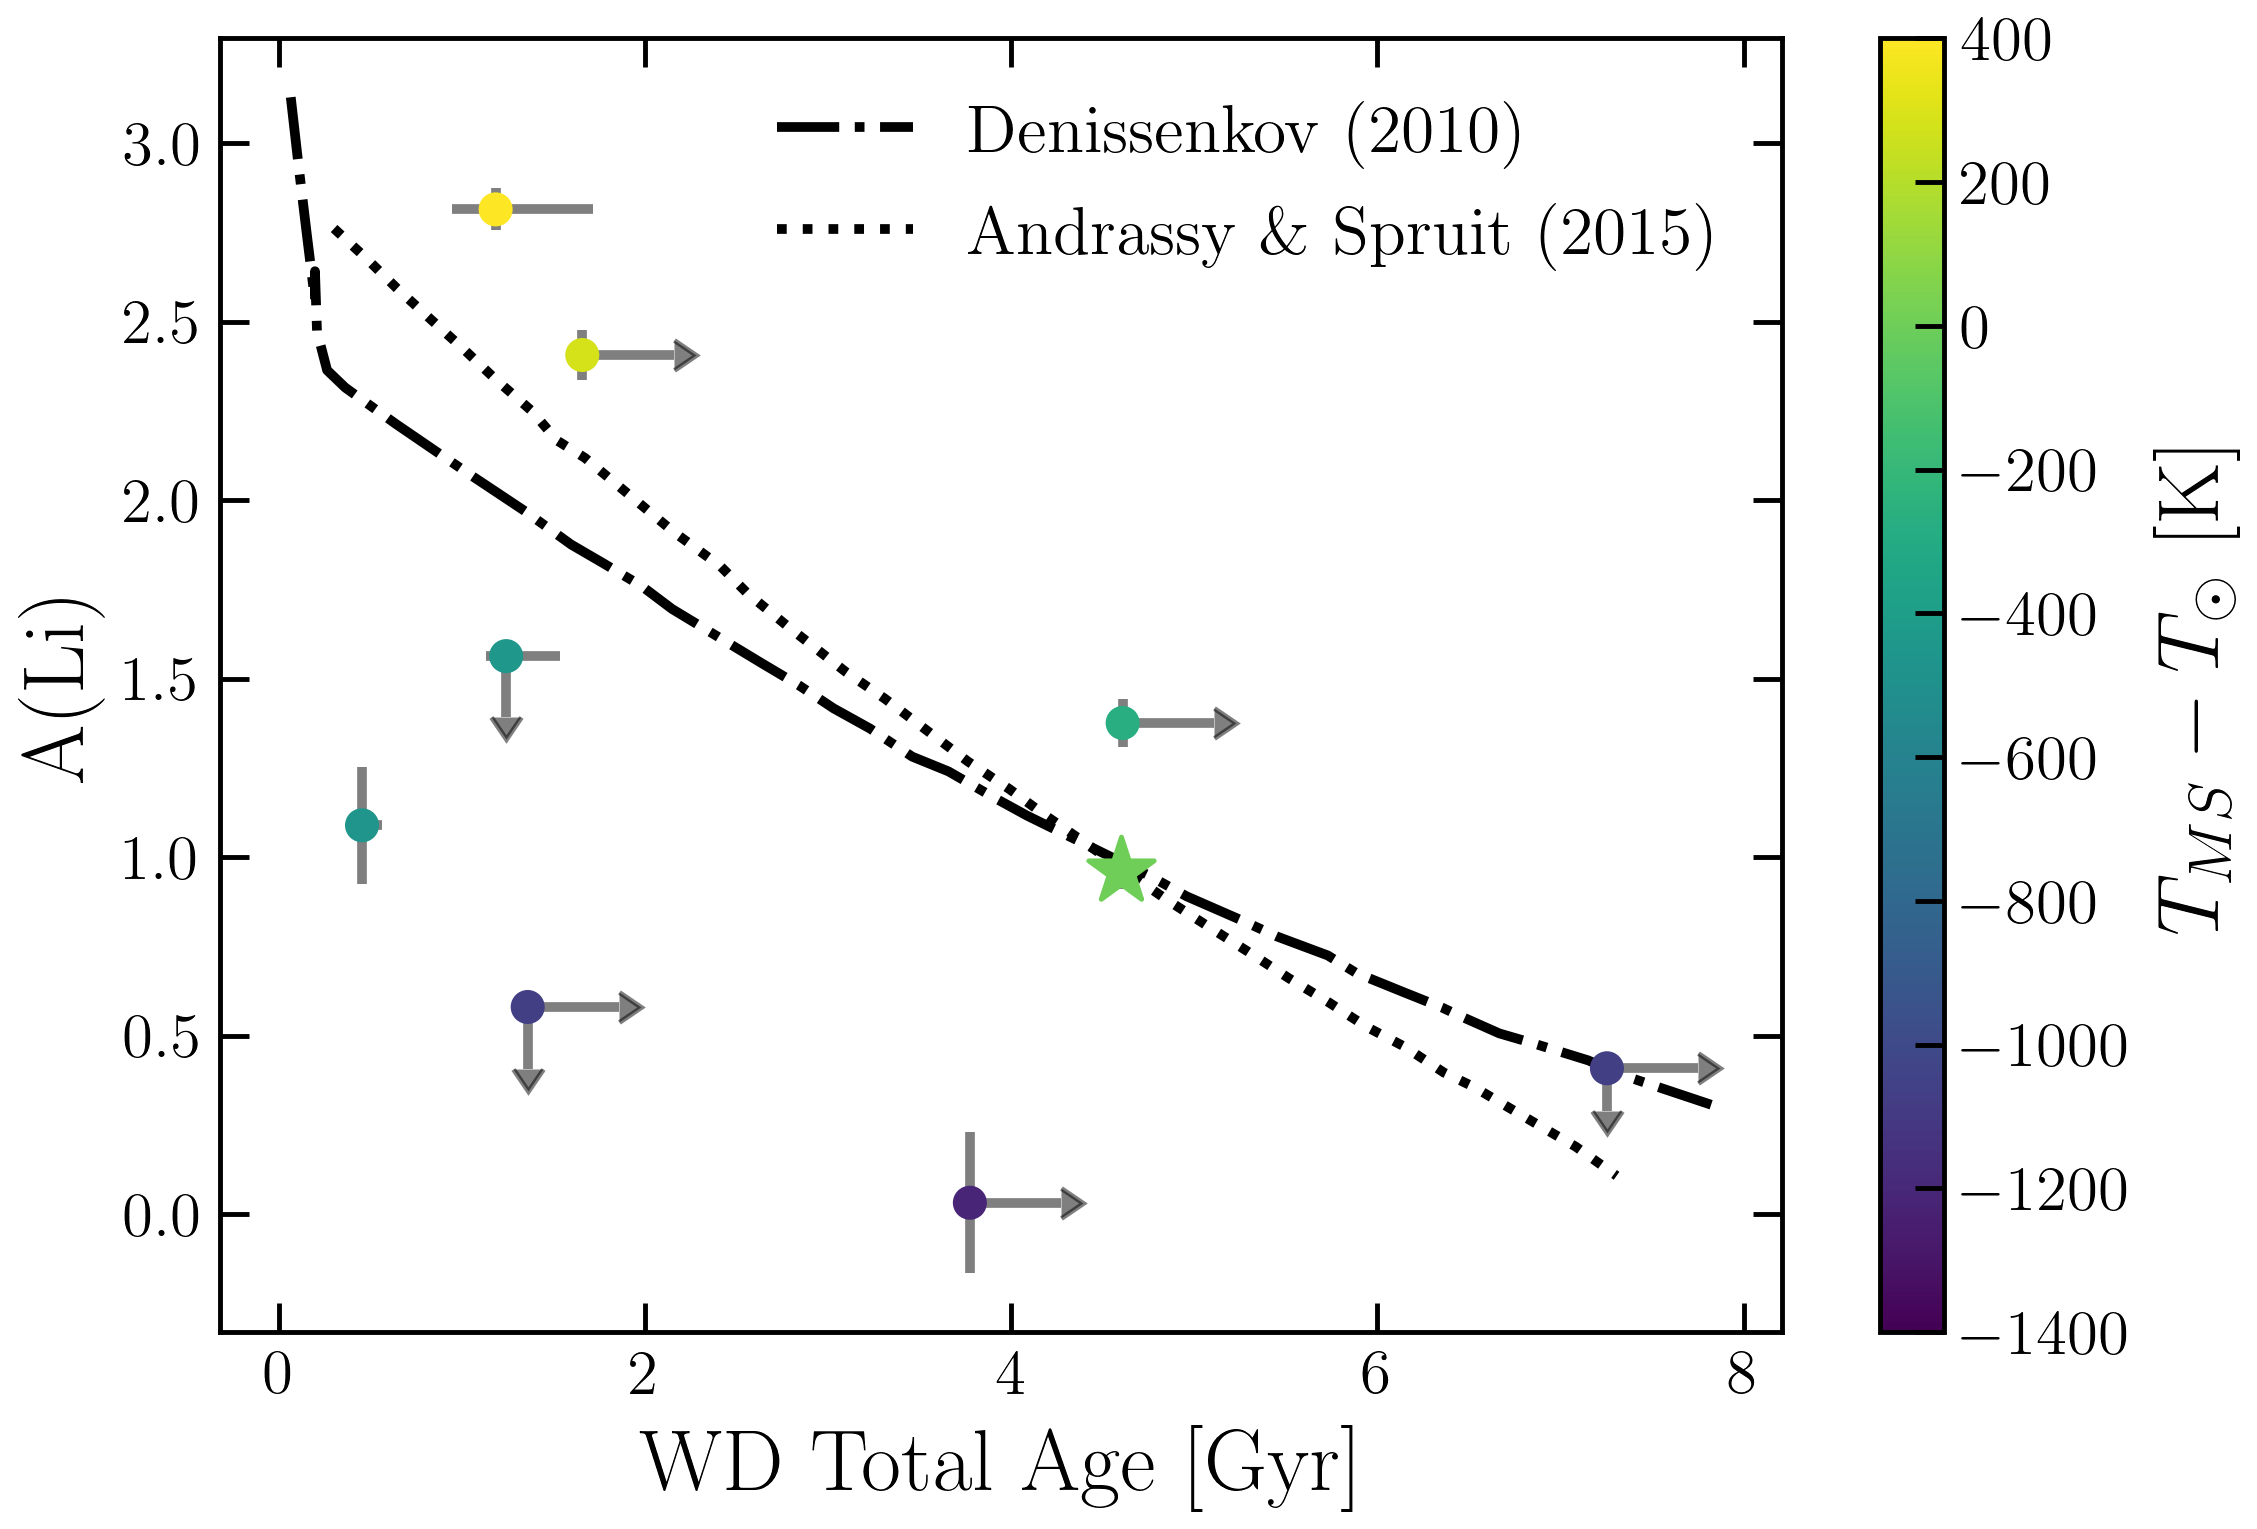
\includegraphics[width=\columnwidth]{lithium_vs_age.png}
    \caption{Lithium abundance as a function of white dwarf total age. None of the MS components in these systems are solar analogues but models for solar analogues are shown from \cite{2010ApJ...719...28D} and \cite{2015A&A...579A.122A} to show a reasonable expected trend. The Sun's position is shown as a star symbol. There is a general trend of decreasing A(Li) as a function of age.}
    \label{fig:lithium}
\end{figure}

\subsection{$\alpha$-Enhanced and Carbon-Rich Stars}

Through our investigation of metallicities, we are able to determine if certain MS stars are enriched in certain elements like $\alpha$-process elements, particularly carbon. These enhancements can point to the presence of a binary companion and give hints to the effects of the white dwarf's progenitor on its binary companion through mass transfer events (e.g., wind accretion, \citealt{1988A&A...205..155B}). 

To start, we determine which MS stars have $\alpha$ enhancements by plotting $\left[\mathrm{\alpha/H}\right]$ versus $\left[\mathrm{Fe/H}\right]$ (see Figure~\ref{fig:alpha_enhance}). There is a cluster of most of the sample near solar $\left[\mathrm{\alpha/H}\right]$ while there is a portion of the sample with $\left[\mathrm{\alpha/H}\right] > 0.1$~dex. We define a star as $\alpha$ enhanced if its $\left[\mathrm{\alpha/H}\right]$ exceeds $0.1$~dex. As can be seen in Figure~\ref{fig:alpha_enhance}, the separation distribution of the $\alpha$ enhanced stars does not differ significantly from the rest of the population. There is a slight difference in the peak of the two distributions on the order of 50-100~au, but it is unclear whether the white dwarf progenitors' winds have affected the MS companions significantly.

Carbon-enhanced stars are an interesting class of stellar objects. These include dwarf carbon stars (dCs, \citealt{2019ApJ...877...44R}), carbon-enhanced metal poor stars (CEMP, \citealt{2007ApJ...655..492A, 2012ApJ...747....2L}), and CH stars \citep{1995MNRAS.277.1443H} among others. It is widely believed that these carbon enhanced stars are the result of binary star systems \citep[e.g.,][]{2005ApJ...625..825L}, but at separations smaller than the ones in our wide binary sample. When looking at these carbon enhancements, we find the that the carbon-enhanced stars are preferentially in wider orbits (see Figure~\ref{fig:carbon_enhance}). If the carbon-enhancements came from the white dwarf progenitor, then it would be expected to affect the smallest separations. Instead, it appears these carbon-enhanced stars are getting their enhancements from another close binary companion, making these systems triples. It is known that hierarchical systems are more stable and dissipate on longer timescales than non-hierarchical systems \citep{1983ApJ...268..319H}. This is in line with our finding that the carbon-enhanced stars are in wider orbits, allowing for a larger parameter space of long-term stable orbits. More work with high-resolution spectra is needed to confirm the true nature of these systems, but they provide an interesting subset for future study.

The last class of stars we investigate is barium (Ba) stars \citep{1951ApJ...114..473B, 2019A&A...626A.127J}, which are hypothesized and observed to form in binaries through mass transfer events \citep{1990ApJ...352..709M,1995MNRAS.277.1443H}. The presence of any Ba stars in the sample would indicate mass transfer from an AGB star occurred and could help place constraints on the level of wind accretion in these wider binaries. Figure~\ref{fig:Ba_enhance} shows the barium abundances in our sample as a function of metallicity. There is only one star (HD 72223) with $\left[Ba/Fe\right] > 1.0$~dex (a rough estimate of the level of enhancement needed to classify as a Ba star). HD 72223 is a known spectroscopic binary with a close companion identified in Gaia DR3 \citep{2023A&A...674A..34G}, which is responsible for its enhanced Ba abundance. This shows that it is unlikely that any significant wind accretion is occurring during the AGB phase of the white dwarfs in the wide WD+MS sample.

\begin{figure}
    \centering
    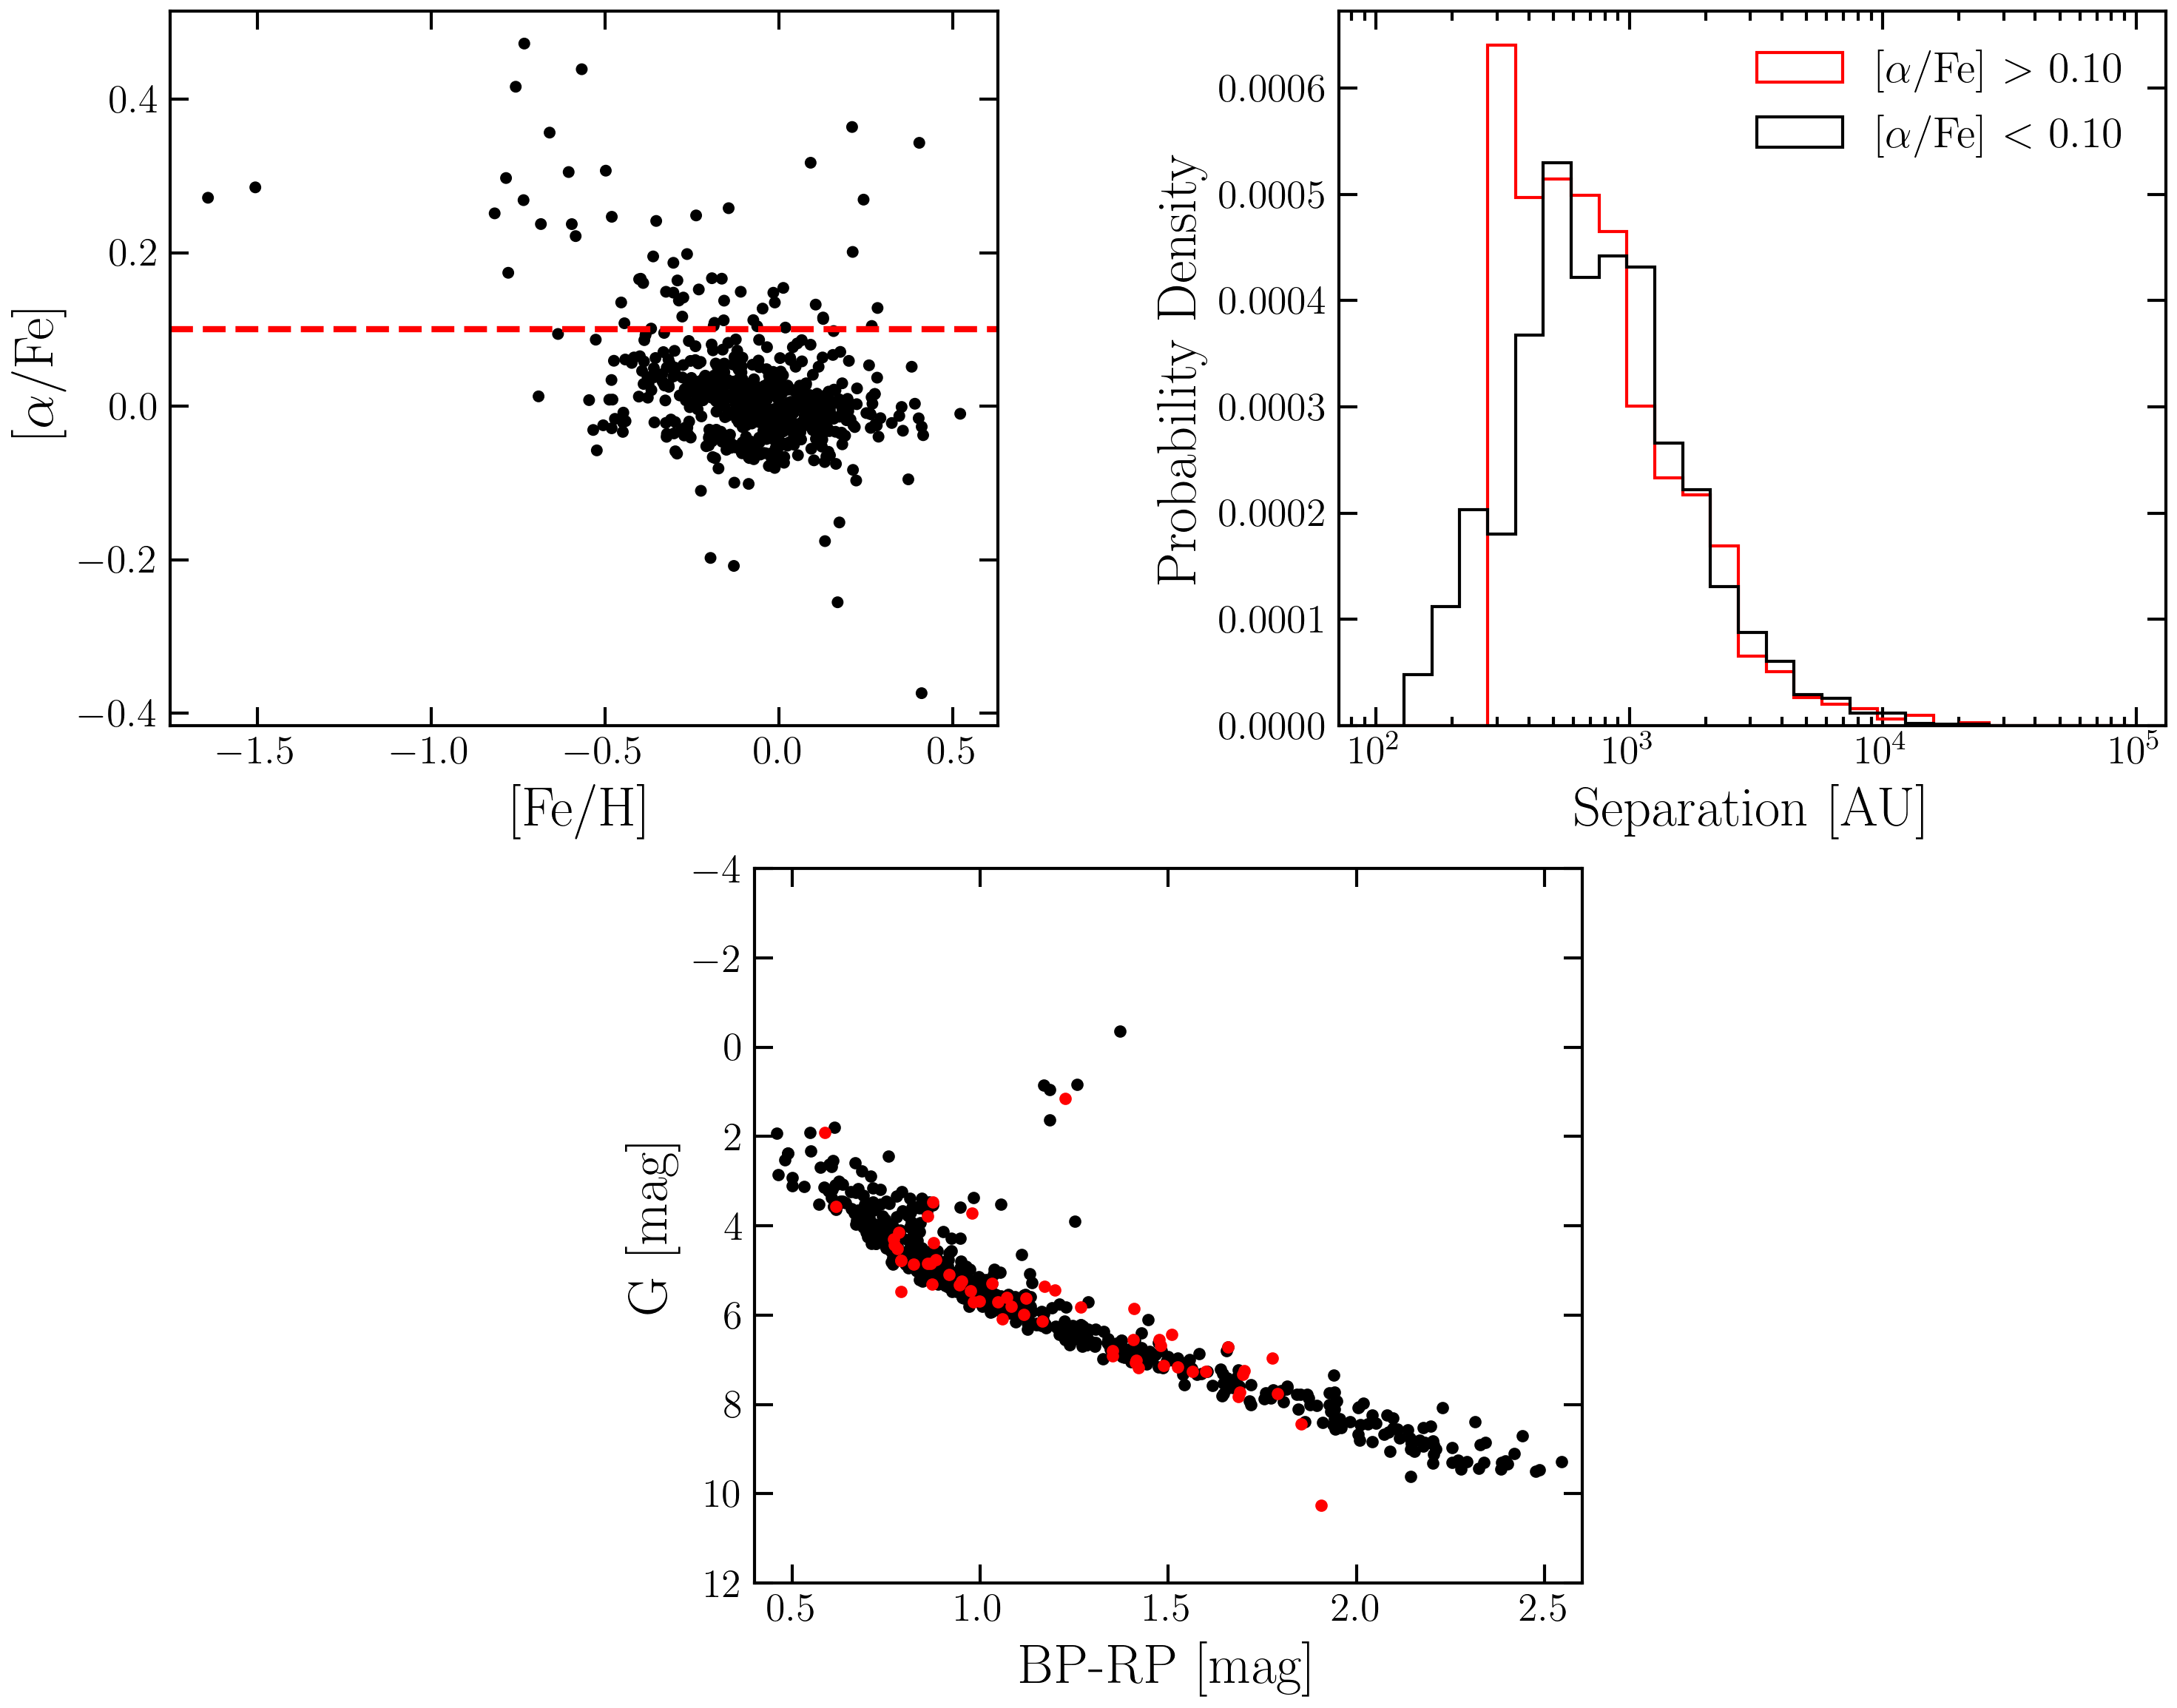
\includegraphics[width=\columnwidth]{alpha_enhance.png}
    \caption{$\alpha$ enhanced stars in the wide WD+MS binary sample. The upper left panel shows $\alpha$ abundances versus metallicity with the red dashed line denoting the cutoff for our definition of $\alpha$ enhanced. The upper right panel shows the separation distribution of the $\alpha$ enhanced (red) and non-$\alpha$ enhanced stars (black). The $\alpha$ enhanced stars do not show any significant differences in their separation distribution. The bottom panel shows a Gaia CMD of the $\alpha$ enhanced (red) and non-$\alpha$ enhanced stars (black). The majority of the $\alpha$ enhanced stars have main-sequence luminosities.}
    \label{fig:alpha_enhance}
\end{figure}

\begin{figure}
    \centering
    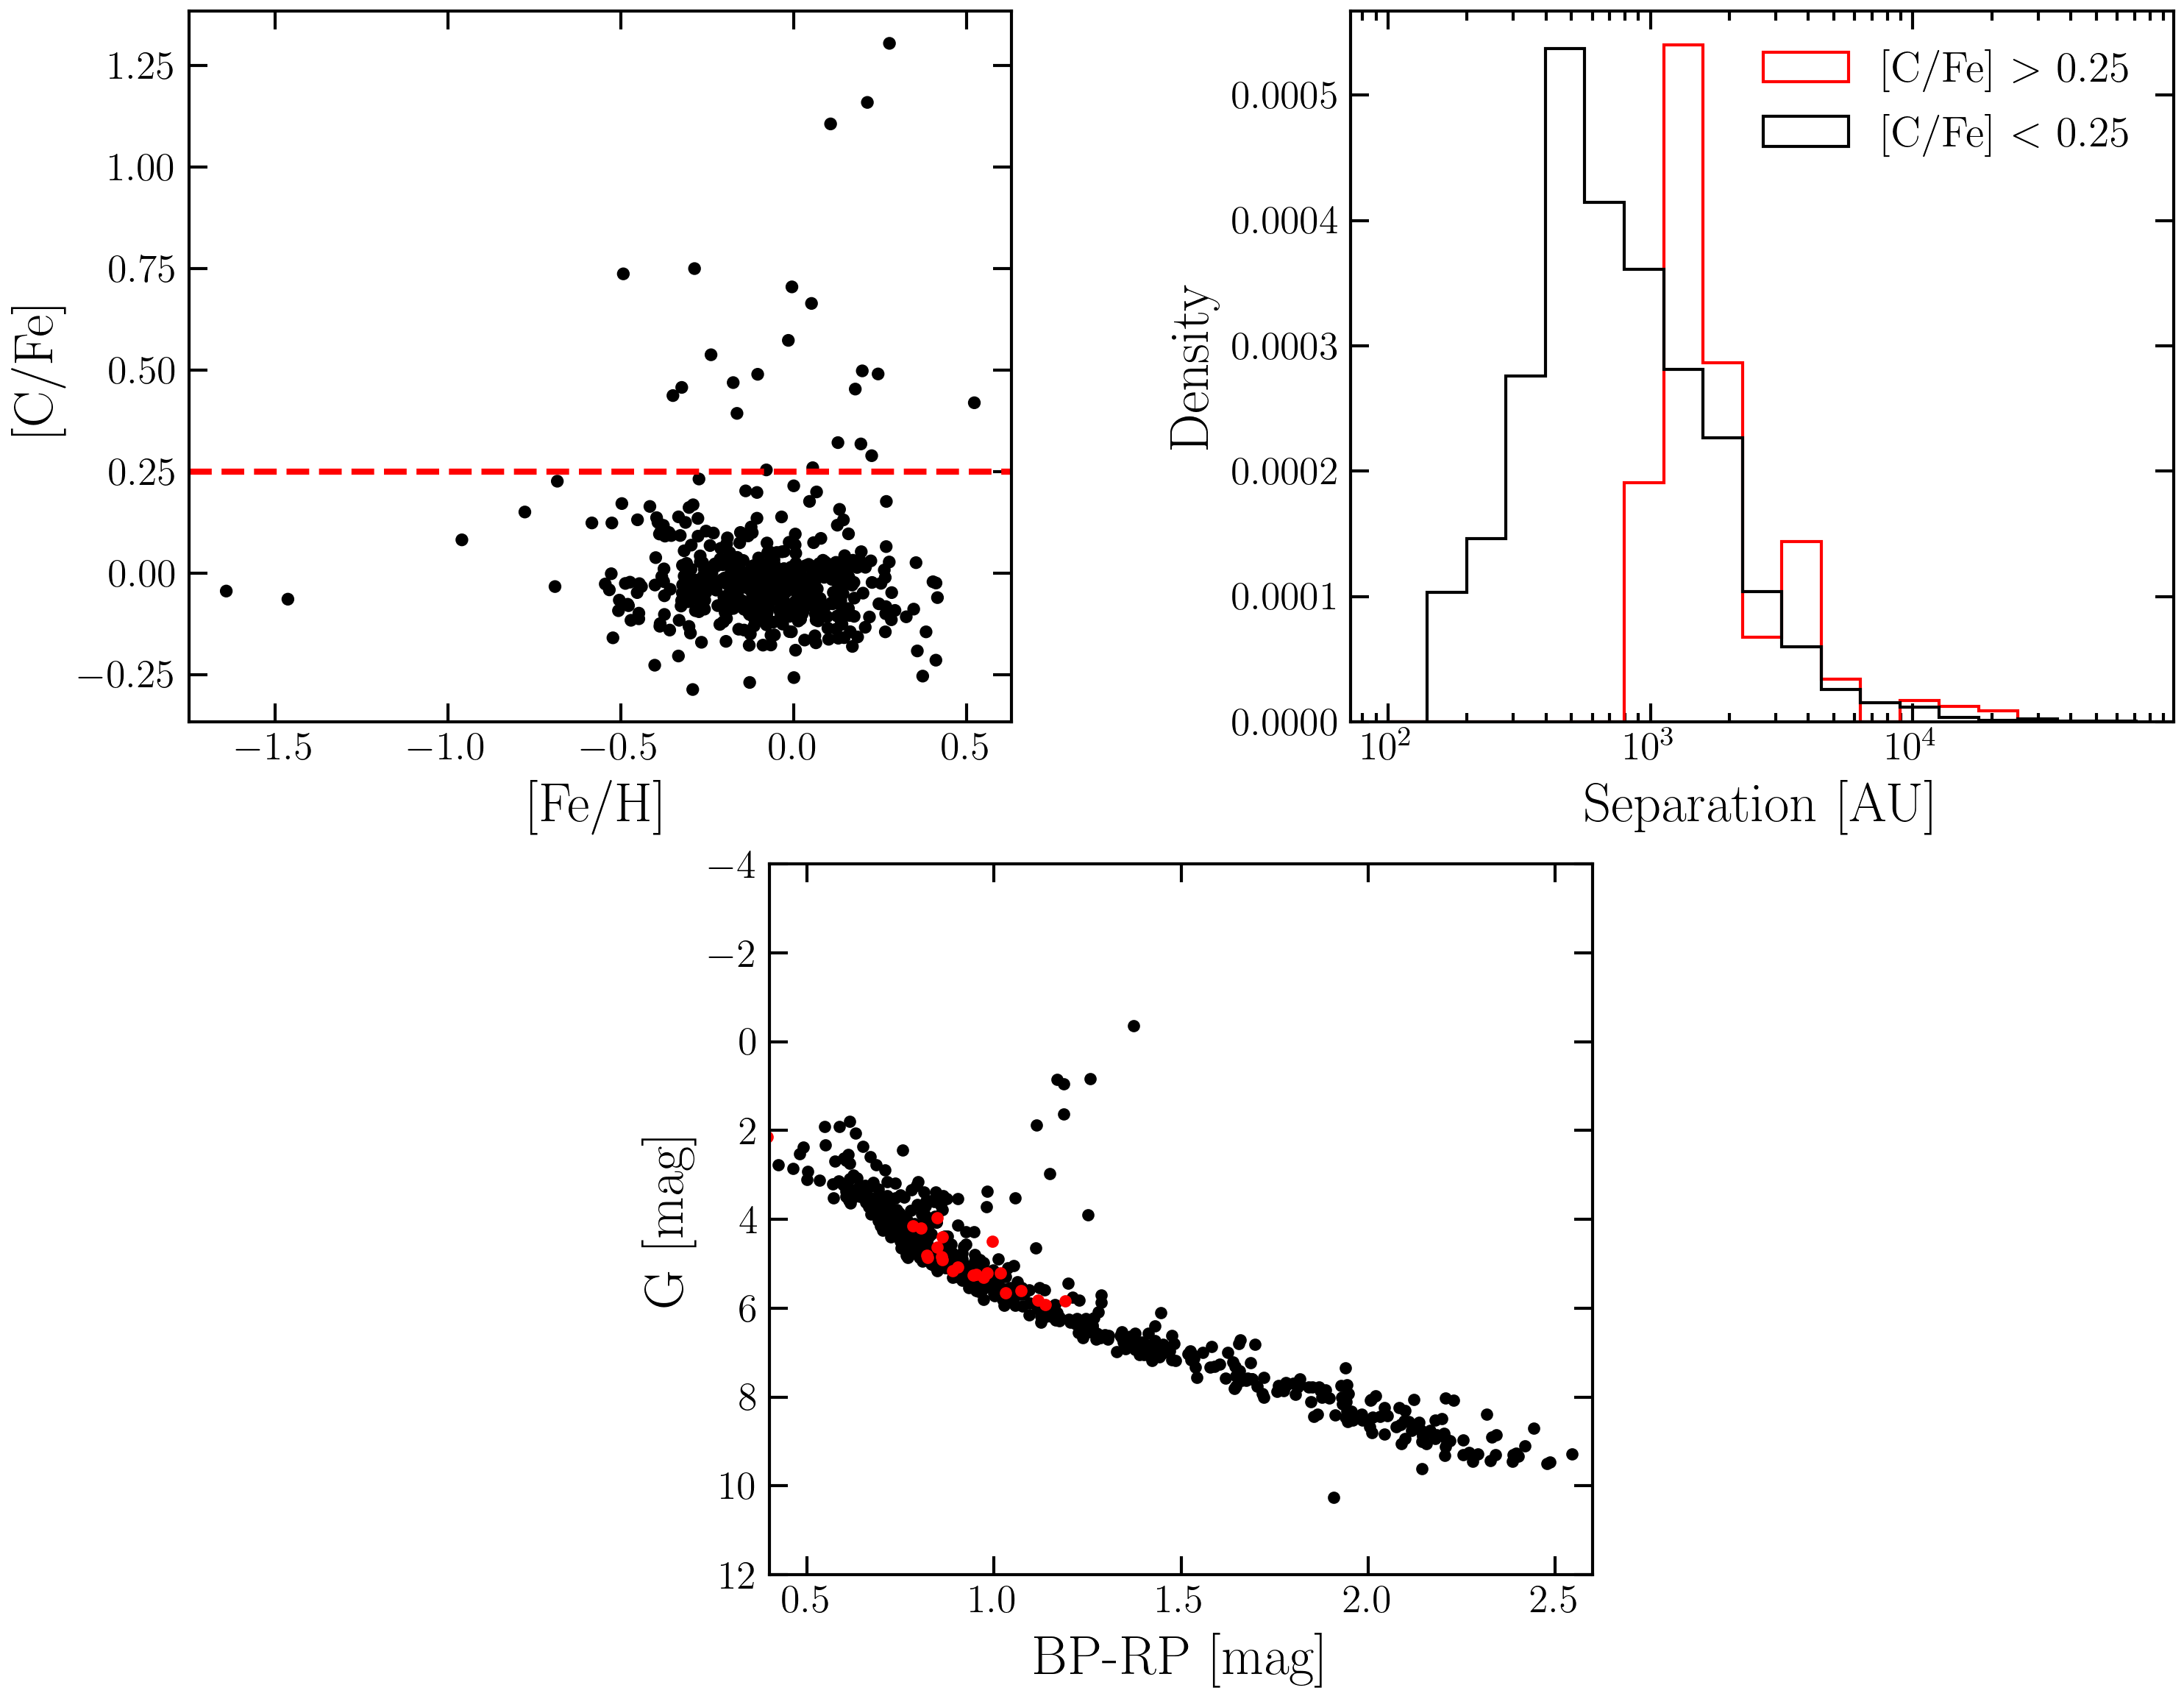
\includegraphics[width=\columnwidth]{C_enhance.png}
    \caption{The same as Figure~\ref{fig:alpha_enhance} but with carbon abundances. The upper right panel shows that the carbon enhanced stars ($\left[\mathrm{C/H}\right] > 0.25$) have larger separations than the non-carbon enhanced stars. The bottom panel shows that all the carbon enhanced stars have main-sequence luminosities.}
    \label{fig:carbon_enhance}
\end{figure}

\begin{figure}
    \centering
    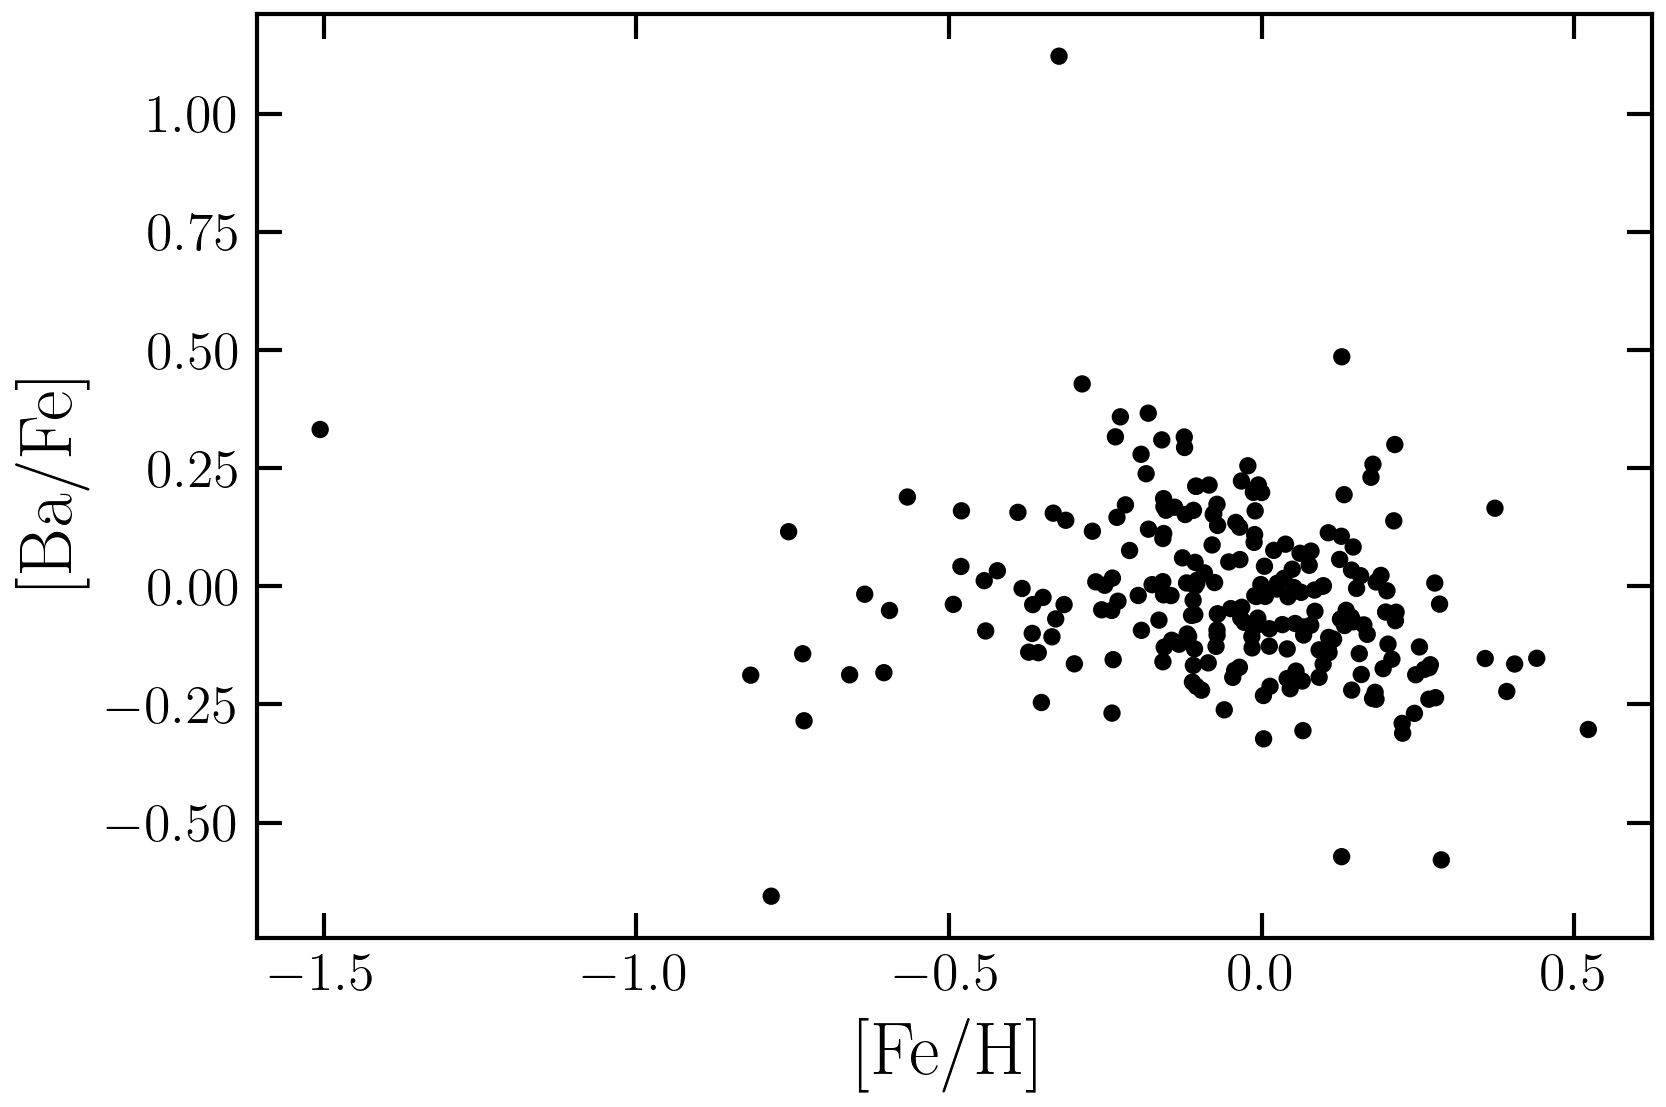
\includegraphics[width=\columnwidth]{Ba_enhance.png}
    \caption{Barium abundances as a function of metallicity. There is only one star (HD 72223) with Ba enhancements at the level of a Ba star ($>1.0$~dex). There is no evidence of AGB wind accretion from the white dwarf progenitors in the wide WD+MS sample.}
    \label{fig:Ba_enhance}
\end{figure}

\subsection{Age-Velocity Dispersion Relation}\label{sec:AVR}

The sample of wide WD+MS binaries provides an opportunity to test the relationship between 2D space velocities and white dwarf age. With the presence of the MS star, more precise parallaxes can be calculated and employed to generate more precise space positions and motions. The weighted mean parallaxes of the sample improve on the precision of the white dwarf parallax by a factor of five on average. 

First, we generate a clean sample of WD+MS binaries that have white dwarf total age uncertainties $<20\%$ and low BP-RP excesses as described in Section~\ref{sec:metal}. We also restrict the sample to white dwarfs above 0.63~\msun\ given the results found in Chapter~\ref{sec:chap2}. Lastly, we restrict the sample to white dwarfs with determined spectral types. This cut ensures that the correct atmospheric models are applied to each white dwarf, removing any systematics from applying the incorrect models. We find when including white dwarfs without known spectral types, the velocity dispersion is much higher than expected, indicating non-DA white dwarfs with incorrect ages are influencing the tail of the distribution where a few outliers can have a large impact. These cuts result in a sample of 181 WD+MS systems. The white dwarfs in this sample span masses from $0.7-1.2$~\msun\ with the majority of the systems concentrated in between $0.7-0.9$~\msun\ . Figure~\ref{fig:vel_dispersion} shows the distribution of velocities for this cleaned sample. An expected velocity distribution is shown in red assuming single star evolution for all white dwarfs. The expected distribution is determined through the AVR from \cite{2019ApJ...886..100C} by taking an average of the expected velocity dispersions in $v_l$ and $v_b$ of each system given the white dwarf total age. It is clear from Figure~\ref{fig:vel_dispersion} that the sample of WD+MS binaries does not follow the expected trend, with higher tangential velocities, that can indicate some white dwarf ages were reset by a merger \citep{2020ApJ...891..160C}.

% \begin{figure}
%     \centering
%     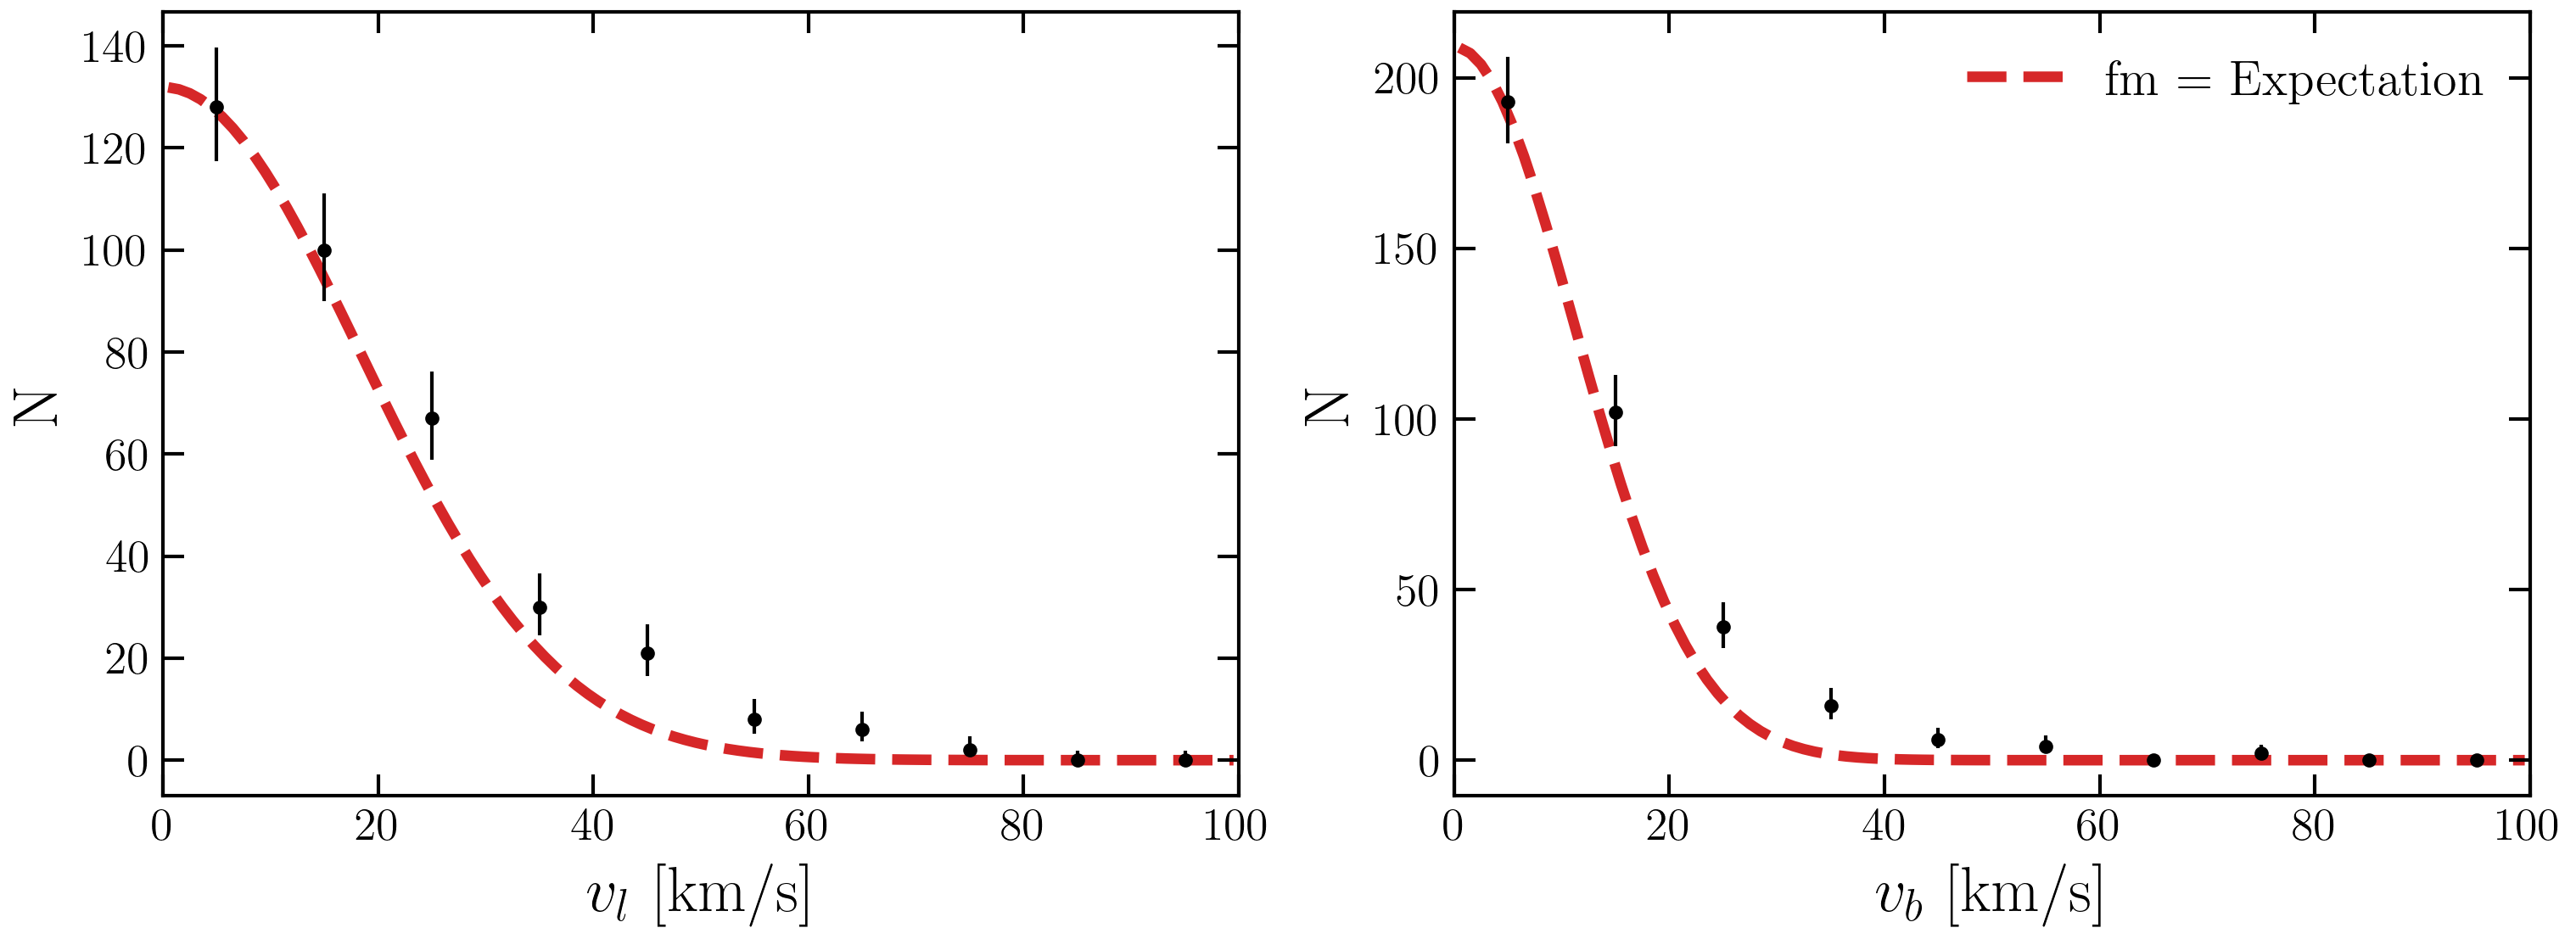
\includegraphics[width=\columnwidth]{vel_dist.png}
%     \caption{The observed velocity dispersion in $v_l$ and $v_b$ for the WD+MS sample described in Section~\ref{sec:AVR} (black points). The expected velocity dispersion given the ages of the white dwarfs in the systems is shown as a dashed red line. Errors are determined through Poisson statistics taken from \cite{1986ApJ...303..336G}.}
%     \label{fig:vel_dispersion}
% \end{figure}

To determine what distribution of ages is needed to reproduce the observed velocity distribution, we calculate the expected velocity dispersion ($\sigma_i$) for a population of stars at constant ages between 0.25 and 10 Gyr with steps of 0.25~Gyr. We fit the observed velocity distributions in $v_l$ and $v_b$ with the following weighted sum;
\begin{equation}
    N_{\mathrm{expected}}(v) = A\sum^{40}_{i=1} w_i \exp{(-v/2\sigma_i)^2}
\end{equation}
where $A$ is a normalization factor, $w_i$ is a weighting factor, and $\sigma_i$ is the expected velocity dispersion of the $i^{\mathrm{th}}$ age. We find that a population of very old ($>7$~Gyr) stars in the sample could explain the discrepancy between the expected and observed velocity distributions at the level of around 30\% (see Figure~\ref{fig:vel_fit}). It is important to note that the fit we have done is highly degenerate, with 40 separate weighting factors being fit. We run the fit 100 times with random starting positions and find the simulated age distribution does not change significantly over the 100 runs.

% \begin{figure}
%     \centering
%     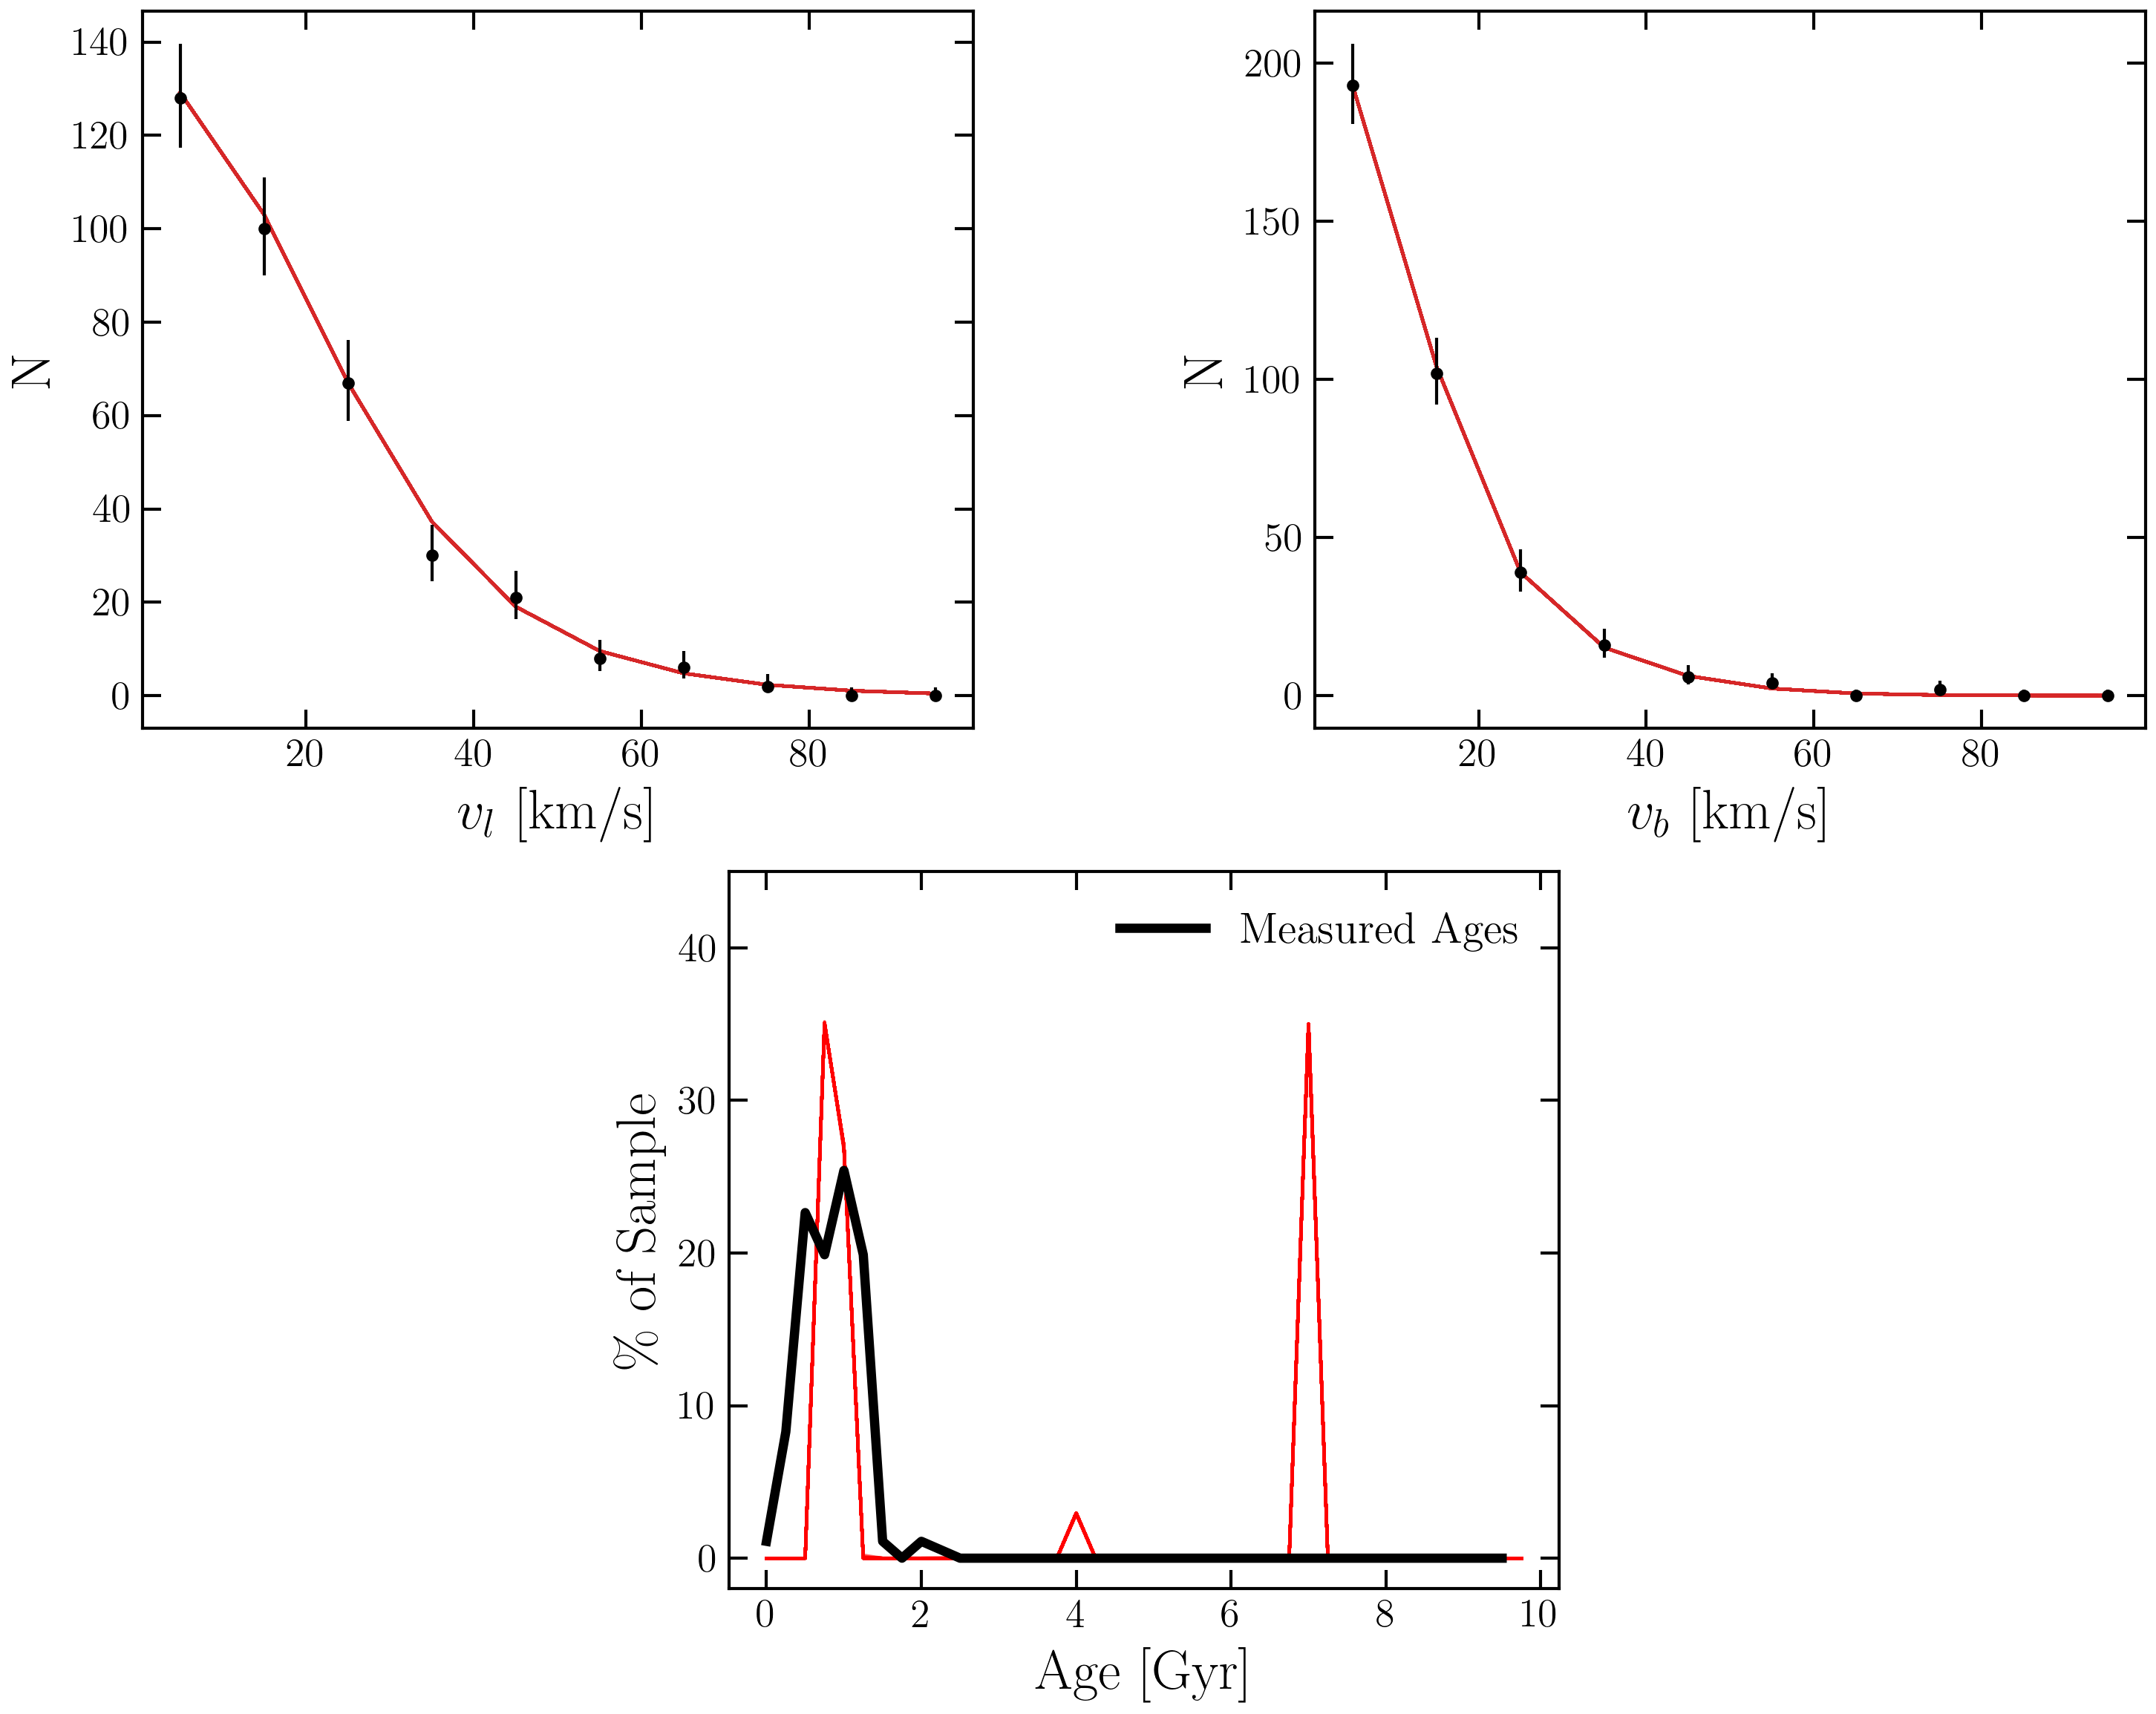
\includegraphics[width=\columnwidth]{vel_fit.png}
%     \caption{A fit to the velocity distributions in $v_l$ and $v_b$ of the sample of WD+MS binaries described in Section~\ref{sec:AVR}. The black points are the observed velocity distribution with errors determined through Poisson statistics taken from \cite{1986ApJ...303..336G}. The red line shows the best fit velocity distribution described in Section~\ref{sec:AVR}. The bottom panel shows the observed age distribution of the sample in black and the corresponding age distribution to produce the best fitting velocity distribution in red. An older population with a larger velocity dispersion is needed to alleviate the discrepancy between the observed and expected velocity distribution shown in Figure~\ref{fig:vel_dispersion}.}
%     \label{fig:vel_fit}
% \end{figure}

Thus, it is clear that a much older population is necessary to reproduce the observed velocities in the sample. There are three possible mechanisms for why the white dwarf ages appear underestimated by such a large factor: (1) the models applied to some of the white dwarfs do not accurately represent their true atmospheric composition, (2) there is a high merger fraction in the sample, or (3) some of the wide binary systems are in fact triples where one of the components has a close binary companion.

In the process of determining the spectral type of each white dwarf, we have used spectral types determined through Gaia XP spectra for 141 white dwarfs in the final sample. These spectral types could be incorrect, especially for non-DA determinations \citep{2024ANA...682A...5V}, but in Chapter~\ref{sec:chap3}, we found the number of incorrect determinations was of order a few percent which is not a large enough fraction to account for the discrepancy. We could also be applying the incorrect models to a subset of the DCs in our sample. The process used for determining which models to use (see Section~\ref{sec:age_determ_WDMS}) is determined through the measured effective temperature of the white dwarf. This approach could be applying the wrong models since there is no way to know the exact atmospheric composition of DC white dwarfs. Assuming the incorrect atmospheric model can induce a systematic mass shift on the order of 15\% \citep{2012ApJS..199...29G}. This in turn could underestimate the progenitor lifetime causing these white dwarfs to appear younger. For a $0.7$\msun\ white dwarf, the progenitor lifetime goes from $\sim0.5$~Gyr to $\sim6$~Gyr for the $0.6$\msun\ white dwarf. This effect is diminished for the higher mass white dwarfs where shifts in the white dwarf mass result in progenitor lifetime changes $<1$~Gyr. Again, this is unable to explain the full discrepancy considering only 6\% of the sample are DC or DZ white dwarfs.

The white dwarf ages could be suspect due to the presence of mergers. As discussed in Chapters~\ref{sec:chap2} and \ref{sec:chap3}, mergers are expected to be present in the sample at the $\sim20\%$ level. These mergers preferentially cause the white dwarf ages to be underestimated. This results in high total age errors especially for double white dwarf mergers \citep[e.g.,][]{2014MNRAS.441..354T, 2020A&A...636A..31T}. \cite{2020ApJ...891..160C} were able to show that for high-mass white dwarfs, a merger fraction of 20\% was able to reproduce the observed dispersion of velocities in their sample. 

It is outside the scope of this dissertation to appropriately model the delay time distribution to determine the merger fraction needed to reproduce the observed velocities in the sample, but Figure~\ref{fig:avr_mergers} shows a simple but imperfect approach to determining the approximate merger fraction. The expected velocity distributions in Figure~\ref{fig:avr_mergers} are determined through applying random age corrections between 0 and 5~Gyr to a percentage of the white dwarf ages corresponding to the merger fraction. Then, just as described above for the expected distribution in Figure~\ref{fig:vel_dispersion}, we take an average of the expected velocity dispersions for each white dwarf given the new updated ages. This demonstrates that mergers with a delay time distribution between 0 and 5~Gyr can reproduce the observed velocities.

% \begin{figure}
%     \centering
%     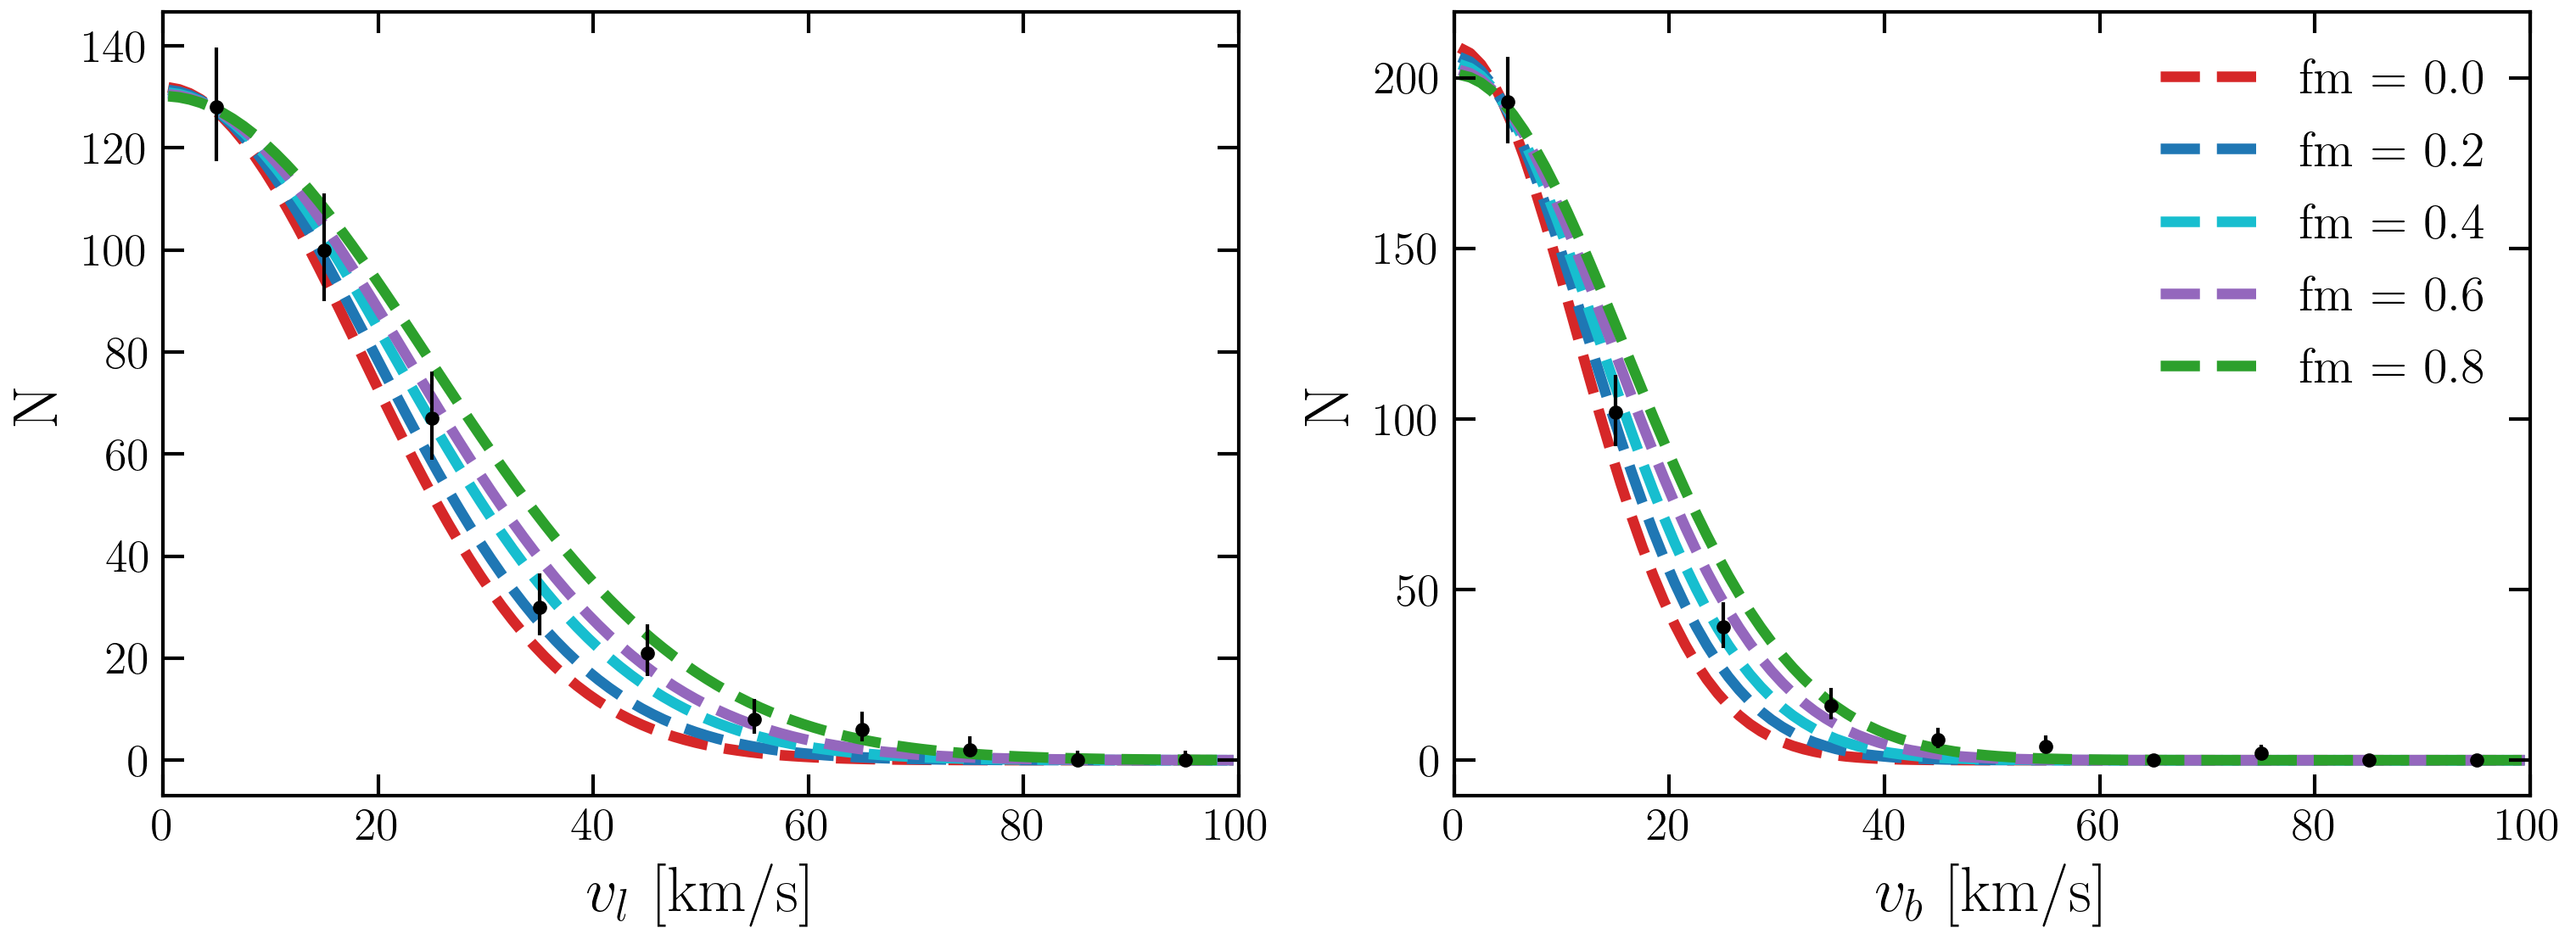
\includegraphics[width=\columnwidth]{vel_dist_mergers.png}
%     \caption{The distribution of velocities in $v_l$ and $v_b$ (black points). Error bars are determined through Poisson statistics taken from \cite{1986ApJ...303..336G}. The expected velocity distributions given a merger fraction are shown as dashed lines.}
%     \label{fig:avr_mergers}
% \end{figure}

Finally, we consider whether a close binary companion to one of the components could be causing issues. The white dwarf could have a close binary companion which is throwing off the SED fit, resulting in incorrect ages. In addition, either the white dwarf or the main-sequence star could have a close binary companion imparting a non-negligible orbital velocity. For the smallest separations in the sample (a few hundred au), the expected circular velocity of the orbit is on the order of a couple km/s. This is not able to explain the observed extra dispersion in the velocities, but if there exist triples in the sample where there is a close binary companion, then the expected orbital velocities begin to approach the level of the observed velocity dispersion with tens of km/s for a separation on the order of one~au.  

It is unclear which of these effects is the largest contributor to the increased velocity dispersion and it is likely that all of these effects are present at some level in the sample.

\section{Discussion and Summary}\label{sec:chap4_conclude}

In this work, we determined ages from all-sky photometry for over 12,000 white dwarfs in wide WD+MS binaries. We gathered spectral types for over 6000 of the white dwarfs in the sample to ensure the employment of appropriate atmospheric models. We also compile $\left[\mathrm{Fe/H}\right]$ measurements for over 500 of the MS components of the WD+MS binaries, as well as measurements of $\alpha$, lithium, and carbon abundances.

Using a sample of wide WD+MS binaries with high-fidelity white dwarf ages, metallicities, and kinematics, the main findings of this work can be summarized as follows:
\begin{itemize}

\item we find that using white dwarf ages, main-sequence stars $\lesssim 5$~Gyr do not show significant trends as a function of $\left[\mathrm{Fe/H}\right]$. There are slight trends for $\left[\mathrm{Fe/H}\right]$ measurements from APOGEE and LAMOST, which show higher-metallicity stars are older on average, but the spread in white dwarf ages at a given metallicity is large ($\sim 1$~Gyr). This is in line with previous work using white dwarfs in wide binaries \citep{2021MNRAS.505.3165R}, finding a lack of an AMR in the solar neighborhood.

\item we find lithium abundances generally follow the expected trend of lower lithium abundances for older stars. This sample is small (eight systems) which makes drawing conclusions difficult. Another complication is that depletion of lithium is dependent on the mass of the main-sequence star. We do not find any systems with high A(Li) and old ages.

\item we find the velocity distribution in the sample is not consistent with the reported white dwarf total ages. The velocity dispersion is too high, indicating a population of systems where their ages are older than the measured white dwarf total ages. We show that merger remnants present in the sample could explain this discrepancy, which has been seen previously among high-mass white dwarfs \citep{2020ApJ...891..160C}. The increased velocity dispersion could also be the result of a population of triples in the sample where there is a close binary companion to one of the components which imparts a large velocity on one of the components. 

\end{itemize}

In this work, we have compiled ages of white dwarfs in wide WD+MS binaries but have not derived any ages of the MS components. In future work, age constraints from the MS component can be used to find discrepancies that can point to evidence of a merger or if any systematics in the white dwarf ages are present. An age constraint from the MS component could also help to provide more accurate age estimates for the system by using a weighted average age \citep[e.g., ][]{2012ApJ...746..102C}. For now, the white dwarf ages in the wide WD+MS sample reveal no significant trends with metallicity outside of lithium abundances for white dwarf ages $\lesssim 5$~Gyr, and their kinematics hint at a significant merger fraction among the white dwarfs in the WD+MS sample.

\section{Acknowledgements}

\bibliography{Bibliography}{}
\bibliographystyle{aasjournal}

\end{document}
